\documentclass{article}


\usepackage{arxiv}

\usepackage[utf8]{inputenc} % allow utf-8 input
\usepackage[T1]{fontenc}    % use 8-bit T1 fonts
\usepackage{hyperref}       % hyperlinks
\usepackage{url}            % simple URL typesetting
\usepackage{booktabs}       % professional-quality tables
\usepackage{amsfonts}       % blackboard math symbols
\usepackage{nicefrac}       % compact symbols for 1/2, etc.
\usepackage{microtype}      % microtypography
\usepackage{lipsum}
\usepackage{siunitx}
\usepackage[linesnumbered,ruled,vlined]{algorithm2e}
\usepackage{float}
\usepackage{amsmath}
\usepackage{enumerate}
\usepackage{cite}
\usepackage{xcolor}
\usepackage{graphicx}
\graphicspath{ {../img/} }

% Table: multiple row
\usepackage{multirow}
% For subfigures environments
\usepackage{subcaption} 

\newcommand{\note}[1]{\textbf{#1}}

\title{Pratical Assignment: Solving PBO Problems with Evolutionary Algorithms}


\author{
 Xiang He\\
  s3627136\\
  \texttt{x.he.4@umail.leidenuniv.nl}\\
  %% examples of more authors
   \And
 Shupei Li\\
  s3430863\\
  \texttt{s.li.18@umail.leidenuniv.nl} \\
  %% \And
 %% Name \\
  %% Student number\\
  %% \texttt{email address} \\
  %% \AND
  %% Coauthor \\
  %% Affiliation \\
  %% Address \\
  %% \texttt{email} \\
  %% \And
  %% Coauthor \\
  %% Affiliation \\
  %% Address \\
  %% \texttt{email} \\
  %% \And
  %% Coauthor \\
  %% Affiliation \\
  %% Address \\
  %% \texttt{email} \\
}

\begin{document}
\maketitle
%% \begin{abstract}
%% Abstract of your report here.
%% \end{abstract}


% keywords can be removed
%\keywords{First keyword \and Second keyword \and More}


\section{Introduction}\label{sec:intro}
% Intro: GA and ES
The evolutionary algorithm is one type of heuristic algorithm. It is inspired by the evolutionary process in nature and can be applied in various fields, such as engineering electrical electronics, automation control systems, etc \cite{2020slowik}. Generally, evolutionary algorithms begin with population initialization, which generates a set of individuals randomly. Then, the population is updated during the iteration until termination conditions are satisfied. Evolutionary algorithms guide the optimization direction via two basic operators, namely variation and selection \cite{2016eiben}. Variation includes recombination and mutation. It encourages the diversity of the population and a greater coverage of the search space. Selection consists of a series of evaluation strategies determining survivors during each epoch. It controls the overall quality of solution candidates and ensures the optimization does not deviate from the correct direction. The alternation between variation and selection simulates the gene inheritance and natural selection that balances between exploration and exploitation. In this assignment, we investigate two representative evolutionary algorithms --- the genetic algorithm and the evolution strategy. Specifically, we apply these two algorithms to solve two pseudo-boolean optimization (PBO) problems.

% F18
The domain of PBO problems is usually defined on (or can be easily transformed into) $\{0, 1\}^n$, where $n$ represents the problem dimension. Meanwhile, the range of the problem is often limited on the field of real numbers $\mathbb{R}$. Given some constraints, our goal is finding a model satisfied $\{0, 1\}^n\rightarrow \mathbb{R}$ that maximizes (or minimizes) the objective function $F$. The first problem we aim to solve is the low autocorrelation binary sequences (LABS) problem. The input $\mathbf{s}$ of the LABS problem is usually defined on $\{-1, 1\}^n$. The objective of the LABS problem is:

\begin{align*}
    \min\ E\left( \mathbf{s} \right) = \sum_{k = 1}^{n - 1}\left( \sum_{i = 1}^{n - k} s_is_{i + k} \right)^2. 
\end{align*}

Or we can also maximize the merit factor equivalently, which is defined as:

\begin{align*}
    \max\ F\left( \mathbf{s} \right) = \frac{n^2}{2E\left( \mathbf{s} \right) }.
\end{align*}

The term $\frac{E(\mathbf{s})}{n}$ is the total energy of $n$ Ising spins $s_i\in\{-1, 1\}, i = 1, \dots, n$ in statistical physics \cite{2016packebusch}. Variants of the LABS problem have application value in fields like communication engineering and applied mathematics. However, our implementation transforms the domain into $\{0, 1\}^n$ to ensure the compatibility of the software environment. The final objective function can be written as:

\begin{align*}
    \max F(\mathbf{x}) &= \frac{n^2}{2 \sum_{k = 1}^{n - 1}\left(\sum_{i = 1}^{n - k} s_i\cdot s_{i + k}  \right)^2 }\\
    s.t.\quad s_i &= 2x_i - 1,\ x_i\in\{0, 1\}, i = 1, \dots, n.
\end{align*}

Figure \ref{fig:intro-labs} shows the largest known merit factors. Factors are confirmed to be optimal solutions when $n \leq 66$.

\begin{figure}[!ht]
 \begin{center}    
     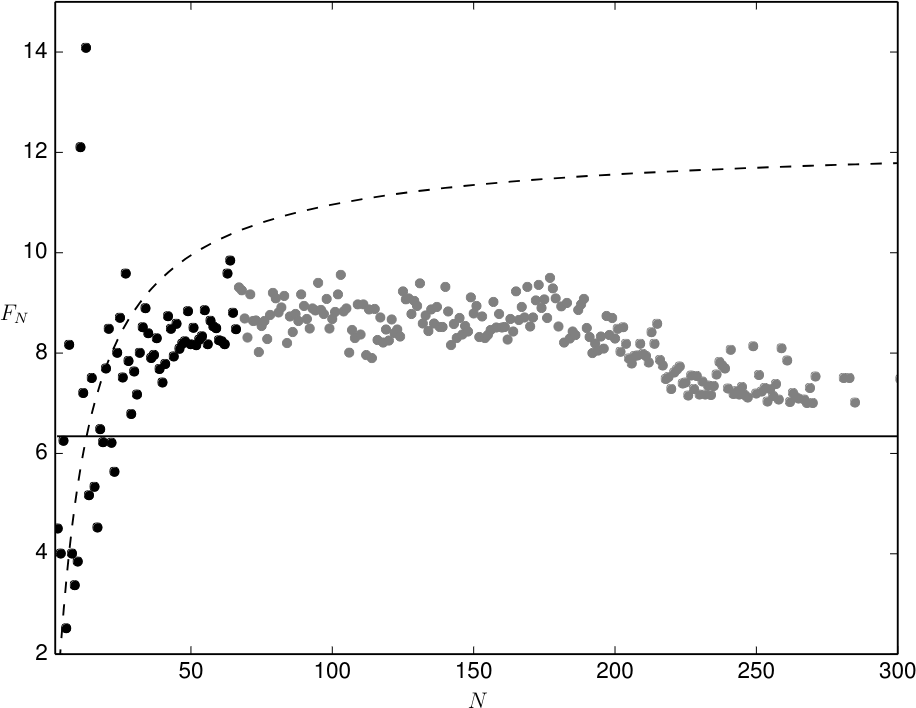
\includegraphics[width=0.5\textwidth]{labs.png}
 \end{center}
 \caption{Largest known merit factors (optimal when $n \leq 66$). This figure is directly adapted from \cite{2016packebusch}.}
 \label{fig:intro-labs}
\end{figure}

% F19
The second problem we focus on in this assignment is the Ising model. The Ising model is an NP-hard problem originating from the ferromagnetism theory. Its general form is defined on an undirected graph $G = \left( V, E \right) $. Each vertex in the graph corresponds to an Ising spin $s_i\in \{-1, 1\}$. Given a weight function $w$, the objective is maximizing $\sum_i\sum_j s_i\cdot s_j \cdot w(e_{ij})$, where $s_i, s_j\in V$ and $e_{ij}\in E$ \cite{2004briest}. In this assignment, we only consider the one-dimensional case, where the structure of the Ising model degenerates to a ring. With assumptions of zero
external magnetic fields and a unit interaction strength, the objective function of the Ising model is:

\begin{align*}
    \max\ F\left( \mathbf{x} \right) = \sum_{i, j, e_{ij}\in E} \left[ x_ix_j + \left( 1 - x_i \right)\left( 1 - x_j \right) \right].
\end{align*}

Notice that the similar transformation trick is applied: $x_i = \frac{s_i + 1}{2}, i = 1, \dots, n$. Consequently, the search space is mapped onto $\{0, 1\}^n$.

% ioh
Our algorithm implementation uses the IOHprofiler framework as the backbone. IOHprofiler integrates many benchmark problems and supports three types of analysis --- fixed-target, fixed-budget, and algorithm parameters \cite{2018doerr}. Two problems we study in this assignment have been added to IOHprofiler's built-in benchmark problems, denoted as F18 and F19 of the PBO class. With the help of the IOHprofiler, it is easy to build pipelines that automatically evaluate evolutionary algorithms' performance. We first record experimental logs via the IOHexperimenter module. After that, we upload logs to a free server running the IOHanalyzer service to obtain the statistical summary as well as results presented by images. All of results in this report are outputs of the IOHanalyzer.

% Structure
The rest of this report is organized as follows. Section \ref{sec:imple} describes the genetic algorithm and the evolution strategy in detail. It also provides information about hyperparameter settings. We report the metrics and experimental results in Section \ref{sec:experi}. This report ends with a brief conclusion and discussion.


\section{Algorithms}
\label{sec:imple}
\subsection{Genetic Algorithm}
\subsubsection{Overview}
\label{subsubsec:overview}
The genetic algorithm is designed for the discrete search space, which usually appears in problems related to combinatorial optimization. The binary encoding is a common choice, i.e., $\mathbf{x}\in \{0, 1\}^n$. Given an objective function $F$, the outline of the genetic algorithm used in this project is shown in Algorithm \ref{al:ga-outline}.

\begin{algorithm}[!ht]
\SetAlgoLined
\SetKwInOut{Input}{Input}\SetKwInOut{Termination}{Termination}

\Input{Budget $B$, \\Problem dimension $n$, \\Population size $\mu$, \\Mutation rate $p_m$, \\Update ratio $\theta$, \\Objective function $F$, \\Tournament size $t_k$, \\Tournament probability $p_k$.}
\Termination{The algorithm terminates when $B \leq 0$.}
\SetKwFunction{FSelection}{Selection}
\SetKwFunction{FCrossover}{Crossover}
\SetKwFunction{FMutation}{Mutation}
\SetKwFunction{FEvaluation}{Evaluation}
\SetKwProg{Fn}{Function}{:}{}
\BlankLine

Initialize the population $\mathcal{D}^{(0)} = \{\mathbf{x}_1, \mathbf{x}_2, \dots, \mathbf{x}_{\mu}\}$ by random sampling, where $\mathbf{x}_i = \left[ x_1, x_2, \dots, x_n \right]^T, i = 1,\dots, \mu$ and $x_j\sim \text{iid}\ \texttt{Bernoulli}\left( 0.5 \right), j = 1, \dots, n$\;
\FEvaluation{$\mathcal{D}^{(0)}$, $F$, $B$}\;
$B_{copy}$ = $B$\;

\BlankLine
\While{$B > 0$}{
    updateNumber = $\mu\cdot \theta$\;
    \tcc{Update the population partially.}
    \While{updateNumber $> 0$}{
        $p_1$, $p_2$ = \FSelection{$\mathcal{D}^{(t)}$, $B$, $B_{copy}$, $t_k$, $p_k$}\;
        $c$ = \FCrossover{$p_1$, $p_2$}\;
        \FEvaluation{$c$, $F$, $B$}\;
        \If{c.fitness > $\mathbf{x}_1$.fitness}{
            Delete $\mathbf{x}_1$ from $\mathcal{D}^{(t)}$\;
            $\mathcal{D}^{(t)}$ = $\mathcal{D}^{(t)}$ $\cup$ $c$\;
            Sort $\mathcal{D}^{(t)}$ in ascending order according to fitness values\;
        }
    }
    \FMutation{$\mathcal{D}^{(t)}$, $p_m$}\;
    \FEvaluation{$\mathcal{D}^{(t)}$, $F$, $B$}\;
    $\mathcal{D}^{(t + 1)} = \mathcal{D}^{(t)}$
}

\BlankLine
\Fn{\FEvaluation{$\mathcal{D}$, $F$, $B$}}{
    \For{$i = 1$ \KwTo $\mathcal{D}$.size}{
        $\mathbf{x}_i$.fitness = $F\left( \mathbf{x}_i \right) $\;
        $B$ = $B$ - 1\;
    }
    Sort $\mathcal{D}$ in ascending order according to fitness values\;
}
\caption{Overview of Genetic Algorithm}\label{al:ga-outline}
\end{algorithm}

In the vanilla genetic algorithm, offspring are generated by applying the selection, crossover, and mutation operators sequentially at time $t$. Then, the population at time $t + 1$ is a copy of these offspring. However, we found that updating the whole population at each time step often leads to an unstable performance in pilot experiments. The reason is that the overall population quality may decrease during the optimization since there is no guarantee that offspring have higher fitness values than parents. A decline in the population quality caused by offspring generation is not a big problem with a sufficient budget and a relatively small problem dimension. The decrease in quality at the early stage usually means a broader exploration area in search space and can be compensated easily later. But given $B = 5,000$ and $n = 50$, the convergence rate of the vanilla genetic algorithm is too slow to find a satisifying solution when the budget runs out. To overcome this weakness, we improve the vanilla genetic algorithm in several aspects:

\begin{itemize}
    \item Introduce a hyperparameter update ratio $\theta$ to control the proportion of updating population at each time step. $\theta = 1$ corresponds to the vanilla genetic algorithm, while $\theta = \frac{1}{\mu}$ means only update one individual.
    \item Maintain the ascending order of the population based on the fitness value. An offspring will only be by added to the population if its fitness value is better than the first individual's.
    \item Design a hybrid selection strategy that will be described in Section \ref{subsubsec:selection}. Outputs of the selection operator are two individuals set as parents.
    \item Use an inner loop to generate the offspring one by one until the update ratio is satisfied at each time step, aiming at saving budget and encouraging diversity.
\end{itemize}

The following three sections introduce selection, crossover, and mutation operators used in Algorithm \ref{al:ga-outline} in detail.

\subsubsection{Selection}\label{subsubsec:selection}
There are various selection strategies for the genetic algorithm. The different strategies put different selection pressures on the population during optimization. Here, we mainly consider three representative selection strategies and develop a hybrid selection operator. Algorithm \ref{al:ga-selection} illustrates the idea of combining different selection strategies.

\begin{algorithm}[!ht]
\SetAlgoLined
\SetKwProg{Fn}{Function}{:}{}
\SetKwFunction{FSelection}{Selection}
\SetKwFunction{FPropSelection}{ProportionalSelection}
\SetKwFunction{FRankSelection}{RankSelection}
\SetKwFunction{FTourSelection}{TournamentSelection}
\BlankLine

\Fn{\FSelection{$\mathcal{D}$, $B$, $B_{copy}$i, $t_k$, $p_k$}}{
    $B_{current}$ = $B_{copy} - B$\;
    \uIf{$B_{current} < (0.4\ast B_{copy})$}{
        \FPropSelection{$\mathcal{D}$}\tcp*{Early stage: proportional selection.}
    }
    \uElseIf{$B_{current} < (0.6 \ast B_{copy})$}{
        \FRankSelection{$\mathcal{D}$}\tcp*{Middle stage: rank selection.}
    }
    \Else{
        \FTourSelection{$\mathcal{D}$, $t_k$, $p_k$}\tcp*{Late stage: tournament selection.}
    }
    Sample two individuals $p_1, p_2$ without replacement from $\mathcal{D}$ by simple random sampling, where $P(\mathbf{x}\text{ is selected}) = \mathbf{x}$.p\_selection\;
    \Return{$p_1, p_2$}
}

\BlankLine
\Fn{\FPropSelection{$\mathcal{D}$}}{
    sum = 0\;
    \ForEach{$\mathbf{x}\in\mathcal{D}$}{
        sum = sum + $\mathbf{x}$.fitness\;
    }
    \ForEach{$\mathbf{x}\in\mathcal{D}$}{
        $\mathbf{x}$.p\_selection = $\mathbf{x}$.fitness / sum\;
    }
}

\BlankLine
\Fn{\FRankSelection{$\mathcal{D}$}}{
    \tcc{$\mathcal{D}$ is sorted based on fitness.}
    \For{$i = 1$ \KwTo $\mathcal{D}$.size}{
        $\mathbf{x}_i$.p\_selection = $(2\ast i) / (\mathcal{D}.\text{size}\ast (\mathcal{D}.\text{size} + 1))$\;
    }
}

\BlankLine
\Fn{\FTourSelection{$\mathcal{D}$, $t_k$, $p_k$}}{
    Sample $t_k$ individuals from $\mathcal{D}$ to constitute $\mathcal{D}_{tour}$. For other non-selected individuals, $\mathbf{x}$.p\_selection = 0\;
    Sort $\mathcal{D}_{tour}$ in descending order according to fitness values\;
    \For{$i = 1$ \KwTo $\mathcal{D}_{tour}$.size}{
        $\mathbf{x}_i$.p\_selection = $p_k(1 - p_k)^i$\;
    }
    Normalize the selection probabilities\;
}
\caption{Genetic Algorithm: Hybrid Selection Operator}\label{al:ga-selection}
\end{algorithm}

Proportional selection assigns a selection probability to each individual that is proportional to the fitness. The intuition behind this strategy is the survival of the fittest. However, the proportional selection is likely affected by significant variations in $F$, which may lead to the local optimum trap. Rank selection is a selection strategy that is more robust to the variance. It decides selection probabilities based on a function of the ranking. Here, we adopt the ranking function suggested by \cite{2012cs}:

\begin{align*}
    P\left( \mathbf{x}_i\text{ is selected} \right) = \frac{2r_i}{\mu(\mu + 1)}.
\end{align*}

where $r_i$ is the rank of the individual $x_i$ based on its fitness value in ascending order, and $\mu$ is the population size. Tournament selection is another commonly used strategy. Given a pre-defined tournament size $t_k$ and the tournament probability $p_k$, it firstly samples $t_k$ individuals from the population. Then, the selected individuals compete for the parent qualification following the Geometric distribution with the success probability equal to $p_k$. In other words, the $i$-th fittest individual is assigned the selection probability $p_k\left( 1 - p_k \right)^i $. We apply the normalization to all individuals at the end of the tournament to ensure the sum of selection probabilities equals 1.

The selection pressure of proportional selection, rank selection, and tournament selection increases sequentially. High selection pressure encourages exploitation and reduces exploration, and vice versa. Therefore, we divide the optimization into three stages to balance between exploitation and exploration. The hybrid selection operator can be summarized as follows:

\begin{enumerate}
    \item Early stage: current budget $>$ 0.6 $\times$ total budget. Use the proportional selection to explore the search space.
    \item Middle stage: 0.4 $\times$ total budget $\leq$ current budget $<$ 0.6 $\times$ total budget. Use the rank selection to shift from exploration to exploitation.
    \item Late stage: current budget $\leq$ 0.4 $\times$ total budget. Use the tournament selection to exploit current optimal solutions.
\end{enumerate}

\subsubsection{Crossover}
We choose the one-point crossover operator in the genetic algorithm. Algorithm \ref{al:ga-crossover} and Figure \ref{fig:al-ga-crossover} show the logic of this operator.

\begin{algorithm}[!ht]
\SetAlgoLined
\SetKwProg{Fn}{Function}{:}{}
\SetKwFunction{FCrossover}{Crossover}
\BlankLine
\Fn{\FCrossover{$p_1, p_2$}}{
    Generate a random integer $m \in \{1, 2, \dots, p_1.\text{length}\} $\;
    $c = p_1[:m] + p_2[m + 1:]$\;
    \Return{c}
}
\caption{Genetic Algorithm: One-point Crossover Operator}\label{al:ga-crossover}
\end{algorithm}

\begin{figure}[!ht]
 \begin{center}    
     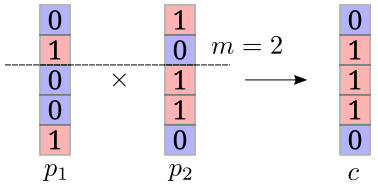
\includegraphics[width=0.5\textwidth]{ga/ga-crossover.png}
 \end{center}
 \caption{One-point crossover operator. Assume $m = 2$.}
 \label{fig:al-ga-crossover}
\end{figure}

Inputs of crossover operator are two parents $p_1 = \left[x_1, x_2, \dots, x_n \right]^T$ and $p_2 = \left[ y_1, y_2, \dots, y_n \right]^T$. The crossover point is generated by sampling an integer $m\in\{1, 2, \dots, n\}$. The child $c$ is produced by swapping bits between parents based on the crossover point, that is, $c = \left[x_1, \dots, x_m, y_{m + 1}, \dots, y_n  \right]^T $. Traditionally, the crossover operator will output two children. However, we only retain the first child because we update the population partially in the genetic algorithm. Redundant offspring will waste valuable budgets.

\subsubsection{Mutation}
\label{subsubsec:mutation}
The mutation operator introduces variations into solutions to broaden the search area in the feasible region. We adopt the bit flip mutation operator because of the usage of binary encoding. The bit flip mutation operator is illustrated in Algorithm \ref{al:ga-mutation} and Figure \ref{fig:al-ga-mutation}.

\begin{algorithm}[!ht]
\SetAlgoLined
\SetKwProg{Fn}{Function}{:}{}
\SetKwFunction{FMutation}{Mutation}
\BlankLine
\Fn{\FMutation{$\mathcal{D}$, $p_m$}}{
    \ForEach{$\mathbf{x}\in\mathcal{D}$}{
        \For{i = 1 \KwTo $\mathbf{x}$.length}{
            Sample $d \sim \texttt{Uniform}(0, 1)$\;
            \If{$d < p_m$}{
                $x_i$ = $|x_i - 1|$\;
            }
        }
    }
}
\caption{Genetic Algorithm: Bit Flip Mutation Operator}\label{al:ga-mutation}
\end{algorithm}

\begin{figure}[!ht]
 \begin{center}    
     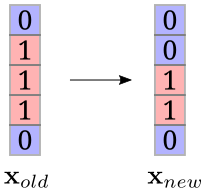
\includegraphics[width=0.28\textwidth]{ga/ga-mutation.png}
 \end{center}
 \caption{Bit flip mutation operator. Assume the second location of the individual is flipped.}
 \label{fig:al-ga-mutation}
\end{figure}

The mutation operator is applied to the whole population. For each location of the individual, the bit flipping happens with probability $p_m$, i.e., $0\rightarrow 1, 1 \rightarrow 0$. With mutation, we can increase the diversity of solutions.

\subsubsection{Hyperparameter Settings}
There are three major hyperparameters in the genetic algorithm --- population size $\mu$, mutation rate $p_m$, and update ratio $\theta$. We perform hyperparameter fine-tuning on these parameters with the grid search method. The fine-tuning results are discussed in Section $\ref{sec:experi}$. As for other hyperparameters, we determine their values according to assignment requirements and the results of pilot experiments. Table \ref{tab:al-ga-hyper} summarizes the hyperparameter settings of the genetic algorithm for reproducibility.

\begin{table}[!ht]
    \centering
    \caption{Hyperparameter settings of the genetic algorithm.}
    \label{tab:al-ga-hyper}
    \begin{tabular}{lll}
       \toprule
       \textbf{Hyperparameter} & \textbf{Meaning} & \textbf{Value}\\
       \midrule
       $B$ & budget & 5,000\\
       $n$ & problem dimension & 50\\
       $t_k$ & tournament size & Equal to the population size\\
       $p_k$ & tournament probability & 0.8\\
       \bottomrule
    \end{tabular}
\end{table}

We set the random seed to 42 when running the genetic algorithm.

\subsection{Evolution Strategy}

Differing from Genetic Algorithms which focus on recombination and selection strategies to find the global optimum in discrete spaces. Evolution Strategies emphasize self-adaptation through mutating with Gaussian perturbations, which achieve convergence in continuous spaces by iterating local optimal selections.

\begin{algorithm}[!ht]
\SetAlgoLined
\SetKwInOut{Input}{Input}\SetKwInOut{Termination}{Termination}

\Input{Budget $B$, \\Problem dimension $n$, \\Population size $\mu$, \\Mutation step-size \( \sigma \), \\Offspring size \( \lambda \), \\Objective function $F$}
\Termination{The algorithm terminates when $B \leq 0$.}
\SetKwFunction{FSelection}{Selection}
\SetKwFunction{FCrossover}{Crossover}
\SetKwFunction{FMutation}{Mutation}
\SetKwFunction{FRecombination}{Recombination}
\SetKwFunction{FEvaluation}{Evaluation}
\SetKwFunction{FConversion}{Gaussian\_to\_uniform}
\SetKwProg{Fn}{Function}{:}{}
\BlankLine

Initialize the population $\mathcal{D}^{(0)} = \{\mathbf{x}_1, \mathbf{x}_2, \dots, \mathbf{x}_{\mu}\}$ by random sampling from normal distribution $\mathcal{N}(0,1)$;

\BlankLine
\While{$B > 0$}{
    $\mathcal{O}$ = \FRecombination{$\mathcal{D}^{(t)}$}\;
    $\mathcal{O}'$ = \FMutation{$\mathcal{O}$, \( \sigma \)}\;
    fitness = \FEvaluation{$\mathcal{D}^{(t)}$ + $\mathcal{O}'$, $F$, $B$}\;
    $\mathcal{D}^{(t+1)}$ = \FSelection{$\mathcal{D}^{(t)}$ + $\mathcal{O}'$, fitness}\;
}

\BlankLine
\Fn{\FEvaluation{$\mathcal{D}$, $F$, $B$}}{
    \For{$i = 1$ \KwTo $\mathcal{D}$.size}{
        $\mathbf{x}_{i}'$ = \FConversion{$\mathbf{x}_i$}\;
        $\mathbf{x}_{i}'$.fitness = $F\left( \mathbf{x}_{i}' \right) $\;
        $B$ = $B$ - 1\;
    }
    Sort $\mathcal{D}$ in ascending order according to fitness values\;
}

\BlankLine
\Fn{\FConversion{$\mathbf{x}_i$}}{
    $\mathbf{x}_{i}'$ = st.norm.cdf($\mathbf{x}_{i}$)\;
    \For{$j = 1$ \KwTo $\mathbf{x}_{i}'$.size}{
        \If{$\mathbf{x}_{i}'[i] \geq 0.5$}{
            $\mathbf{x}_{i}'[i] = 1$\;
        }
        \Else{
            $\mathbf{x}_{i}'[i] = 0$\;
        }
    }
    \KwRet{$\mathbf{x}_{i}'$}\;
}

\caption{Overview of Evolution Strategies}\label{al:es-outline}
\end{algorithm}

Evolution Strategies are designed for real-valued spaces \(\mathbb{R}^n\) in general, which cannot apply to binary problems directly like F18 and F19. Therefore, we implement the evolution strategies on continuous spaces, starting by initializing the populations through random sampling on the normal distribution (0,1). Moreover, we initialize the mutation step sizes (sigma) for each population with a fixed value, which corresponds to our one-step size(sigma) mutation strategies. 

To evaluate the normal distribution populations on binary searching space, we designed a method to convert the Gaussian distribution individual into the binary representation. Function Gaussian\_to\_uniform in Algorithm \ref{al:es-outline} illustrates this conversion.


The function st.norm.cdf() from Scipy applies the cumulative distribution function on individual $\mathbf{x_i}$. Which considers each element in $\mathbf{x_i}$ as an observation value and calculates the cumulative probabilities of the lower or equal to the value in the normal distribution space.  Therefore, we convert the normal distribution values into probability values in the range of [0, 1], and map these values to binary {0, 1} through a threshold of 0.5. Values with probabilities greater or equal to 0.5 are assigned to 1, whereas those below the threshold are mapped to 0. 

\subsubsection{Intermediate Recombination}

\begin{algorithm}[!ht]
\SetAlgoLined
\SetKwProg{Fn}{Function}{:}{}
\SetKwFunction{FRecombination}{Recombination}
\BlankLine
\Fn{\FRecombination{$\mathcal{D}$, \( \lambda \)}}{
    Generating offspring $\mathcal{O} = \{\mathbf{x}_{o1}, \mathbf{x}_{o2}, \dots, \mathbf{x}_{o\lambda}\}$ with the corresponding $ \sigma _{oi}$ for each $x_{oi}$\;

    \For{$i = 1$ \KwTo \( \lambda \)}{
        $x_{p1}$, $x_{p2}$ = $\text{Random select 2 unique individuals from $\mathcal{D}$}$\;
        $x_{oi}$ = $(x_{p1} + x_{p2}) / 2$\;
        $ \sigma _{oi}$ = $(\sigma _{p1} + \sigma _{p2}) / 2$\;
        $\mathcal{O}$ \text{append} ($x_{oi}$, $ \sigma _{oi}$)\;
    }
}

\caption{Evolution Strategies: Intermediate Recombination}\label{al:es-recombine}
\end{algorithm}

Intermediate recombination aims to generate offspring and corresponding mutate step size by calculating the mean value at each operator of two randomly chosen parents as Algorithm \ref{al:es-recombine}. Compared with discrete recombination, this method focuses on generating smoother offspring, emphasizing a stable convergence during the evolutionary process.

\subsubsection{Mutation}

Mutation is an essential part of evolution strategies, which introduce the self-adaptation mechanism into the optimization process. Mutation adds perturbations which randomly sample from the Gaussian distribution to the population. These perturbations allow the algorithm to search on a local solution space. Then we can define the selection function to find the optimal in the local solution space, and iteratively move in that direction until reaching the global optimization. 

Therefore, the mutation step size $\sigma$ and learning rate $\tau$ control the convergence speed of evolution strategies. There we use a one-sigma mutation, which means all search variables in an individual share one sigma. This approach implements a simple adaptation mechanism and reduces the parameter space, which leads to efficient self-adaptation. 


\begin{algorithm}[!ht]
\SetAlgoLined
\SetKwProg{Fn}{Function}{:}{}
\SetKwFunction{FMutation}{Mutation}
\BlankLine
\Fn{\FMutation{$\mathcal{O}$, \( \sigma \)}}{
    Learning rate $\tau = 1.0 / \sqrt{N} $\;
    \For{$i = 1$ \KwTo \( \lambda \)}{
        $\sigma_{oi}'$ = $\sigma_{oi} \times d  \sim  \mathcal{N}(0, \tau)$\;
        \For{$j = 1$ \KwTo $x_{oi}$.length}{
            $x_{oi}[j] = x_{oi} + d'  \sim  \mathcal{N}(0, \sigma_{oi}') $
        }
    }
    Mutate all individuals in offspring $\mathcal{O}$\;
}

\caption{Evolution Strategies: One-\(\sigma\) Mutation}\label{al:es-mutation}
\end{algorithm}

Algorithm \ref{al:es-mutation} illustrates the One-\(\sigma\) Mutation process. For each individual, the step size $\sigma$ is first mutated from a normal distribution according to learning rate $\tau$. Then all variables in the individual are added to a random normal distribution perturbation according to the mutated $\sigma'$.

\subsubsection{Selection}

\begin{algorithm}[!ht]
\SetAlgoLined
\SetKwProg{Fn}{Function}{:}{}
\SetKwFunction{FSelection}{Selection}
\BlankLine
\Fn{\FSelection{$\mathcal{D}$, fitness}}{
    Ranking $x_i$ in $\mathcal{D}$ base on fitness, $i = \{1, 2, \dots, \mu + \lambda\}$\;
    
    $\mathcal{D}^{(t+1)}$ = top $\mu$ $x_i$ in $\mathcal{D}$\;
}

\caption{Evolution Strategies: selection}\label{al:es-selection}
\end{algorithm}

We implement the $(\mu + \lambda)$- selection to rank the individuals both on parents and offspring and select the top -$\mu$ individuals as the parents in the next generation. Which means that we only accept the individuals with improvement. 

\subsubsection{Hyperparameter Settings}
We conducted experiments to optimize three parameters: population size $\mu$, offspring size $\lambda$, and mutation step size $\sigma$. Due to the size of $\lambda$ should always be greater than $\mu$, we used $\lambda_{rate}$ instead. Therefore, the final offspring size should be $\lambda_{rate} * \mu$. Additionally, the impact of different $\lambda_{rate}$ may vary depending on the population size $\mu$. We first experiment with $\mu$ and $\sigma$ to find the best parameter combinations, then experiment with $\lambda_{rate}$ to determine the final parameters. The experiment results are presented in Section $\ref{sec:experi}$. We set a random seed 42 for the code to ensure results can be reproduced. The rest hyper-parameter settings are listed in Table \ref{tab:al-es-hyper}.

\begin{table}[!ht]
    \centering
    \caption{Hyperparameter settings of the evolution strategies.}
    \label{tab:al-es-hyper}
    \begin{tabular}{lll}
       \toprule
       \textbf{Hyperparameter} & \textbf{Meaning} & \textbf{Value}\\
       \midrule
       $B$ & budget & 5,000\\
       $n$ & problem dimension & 50\\
       \bottomrule
    \end{tabular}
\end{table}

\section{Experimental Results}\label{sec:experi}
\subsection{Metrics}
In order to evaluate the models' performance, we choose the following metrics:

\textbf{Statistics}. We report the mean, median, and max of the best-found fitness $f(x)$. Because the objective of both F18 and F19 is maximization, a larger statistic means the better performance.

\textbf{ECDF curves}. We plot the empirical cumulative distribution function of the running time (ECDF). The ECDF curve reflects the proportion of solutions at least as good as a given target $\phi_i$ within the budget $b$.

\textbf{AUC}. We calculate the area under the ECDF curve. AUC measures the overall performance of the algorithm. A higher AUC represents the algorithm performs better on exploration and converges faster.

\textbf{ERT curves}. The expected running time (ERT) curve is widely used in fixed-target analysis. If the algorithm successfully hits the given target $\phi_i$, ERT measures the average time the algorithm needs to find the qualified solution. Otherwise, ERT equals the positive infinity.

We run each experiment 20 times and report the average values of metrics to alleviate the impact of randomness.

\subsection{Genetic Algorithm}
This section first discusses the hyperparameter settings based on fine-tuning results. After that, we report the best result of our implementation of the genetic algorithm with the recommended parameter settings.

We use the grid search method to find suitable parameter settings. If we consider all possible combinations of hyperparameters, the search space is so large that we do not have enough computational resources to exhaust all possibilities. Therefore, our approach is exploring one hyperparameter setting while fixing other parameters.

\subsubsection{Fine-tuning: Population Size}
The population size decides the scale of solutions we keep track of at a specific moment. A large population size increases the diversity of solutions but decreases the number of updates because of the fixed budget. In experiments, we set the population size to 2, 5, 10, 20, and 25. Table \ref{tab:experi-ga-psize} summarizes statistics and AUC values of F18 and F19.

\begin{table}[!ht]
    \centering
    \caption{Summary of statistics and AUC in population size fine-tuning.}
    \label{tab:experi-ga-psize}
    \begin{tabular}{ccccccccc}
        \toprule
        \multirow{2}[3]{*}{Population Size $\mu$} &
        \multicolumn{4}{c}{\textbf{F18}} &
        \multicolumn{4}{c}{\textbf{F19}}\\
        \cmidrule(lr){2-5}
        \cmidrule(lr){6-9}
        & Mean & Max & Median & AUC & Mean & Max & Median & AUC\\
        \midrule
        2   & 2.66 & 3.12 & 2.62 & 0.379 & 31.1 & 38.0 & 30.0 & 0.366\\
        5   & 3.23 & 3.71 & 3.28 & 0.419 & 39.8 & 46.0 & 41.0 & 0.623\\
        10  & 3.70 & \textbf{5.36} & 3.71 & 0.451 & 44.1 & 48.0 & 44.0 & 0.727\\
        20  & \textbf{3.90} & 4.72 & \textbf{3.89} & \textbf{0.464} & \textbf{46.5} & 48.0 & \textbf{46.0} & \textbf{0.763}\\
        25  & 3.72 & 4.45 & 3.71 & 0.446 & 46.0 & \textbf{50.0} & \textbf{46.0} & 0.750\\
        \bottomrule
    \end{tabular}
\end{table}

Figure \ref{fig:experi-ga-psize-ecdf} and Figure \ref{fig:experi-ga-psize-ert} show ECDF and ERT curves, respectively.

\begin{figure}[!ht]
    \centering
    \begin{subfigure}[h]{0.95\linewidth}
        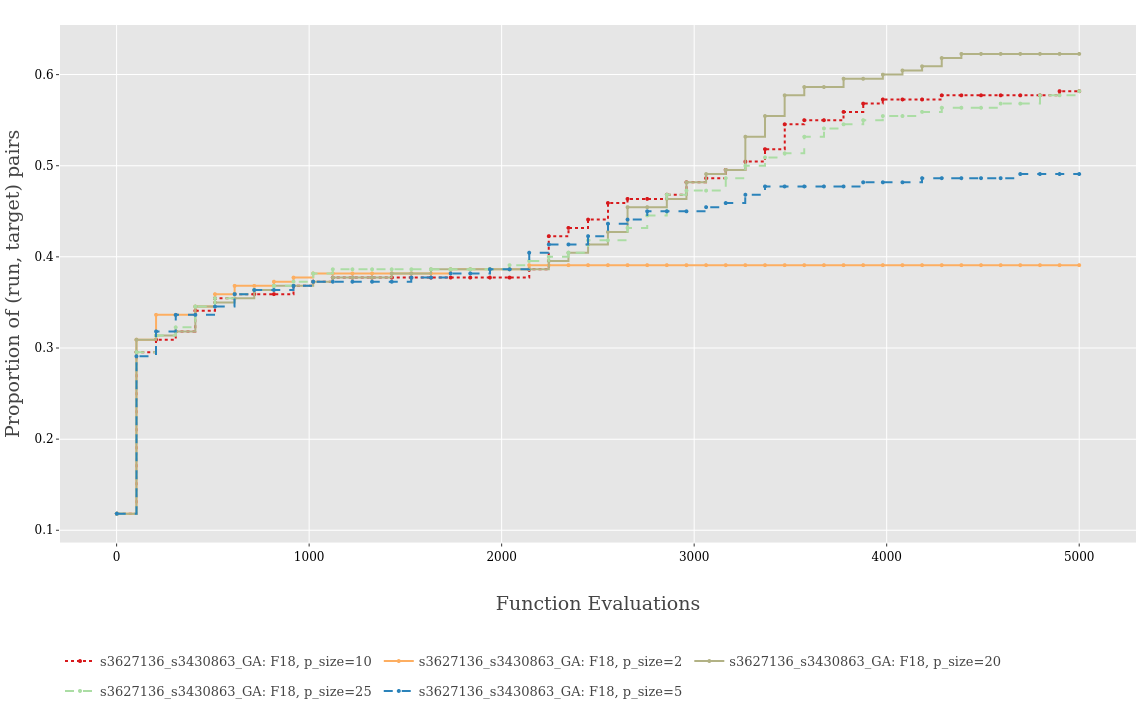
\includegraphics[width=\linewidth]{ga/f18/psize_ecdf.png}
        \caption{GA F18 population size fine-tuning: ECDF curves. $f_{\min} = 0.67, f_{\max} = 5.36, \Delta f = 0.52$.}
    \end{subfigure}
    \hfill
    \begin{subfigure}[h]{0.95\linewidth}
        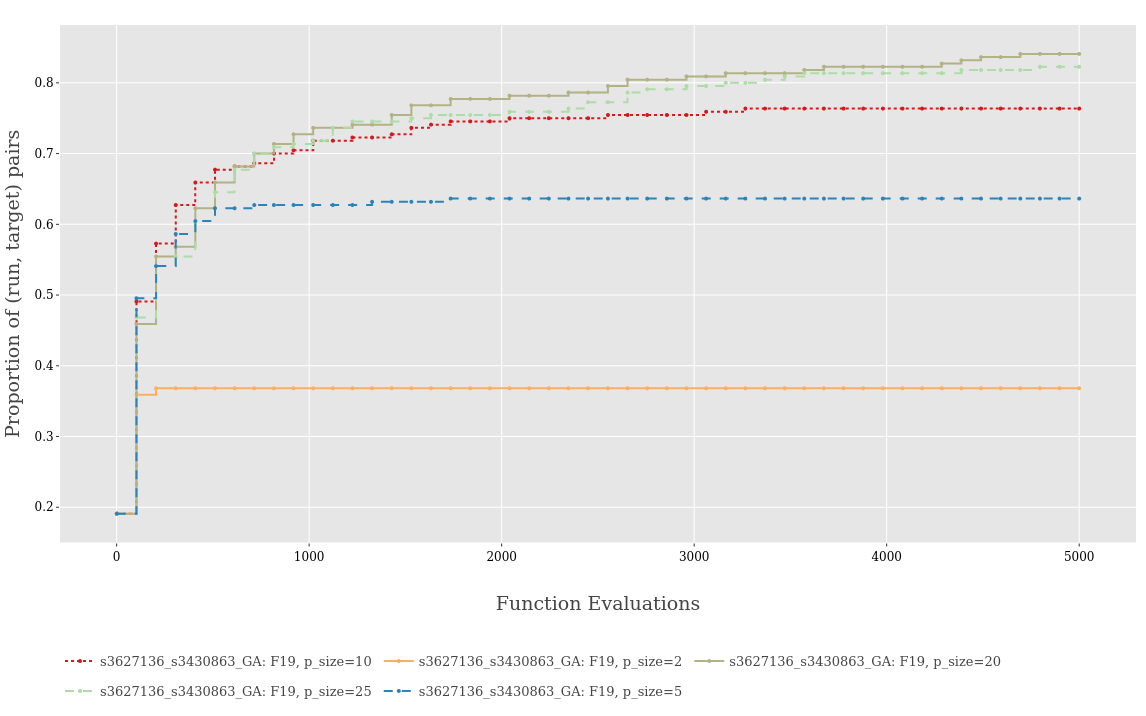
\includegraphics[width=\linewidth]{ga/f19/psize_ecdf.png}
        \caption{GA F19 population size fine-tuning: ECDF curves. $f_{\min} = 20, f_{\max} = 48, \Delta f = 3.11$.}
    \end{subfigure}
    \caption{ECDF curves of the genetic algorithm with various population size settings. Figures are downloaded from the IOHanalyzer.}
    \label{fig:experi-ga-psize-ecdf}
\end{figure}

\begin{figure}[!ht]
    \centering
    \begin{subfigure}[h]{0.95\linewidth}
        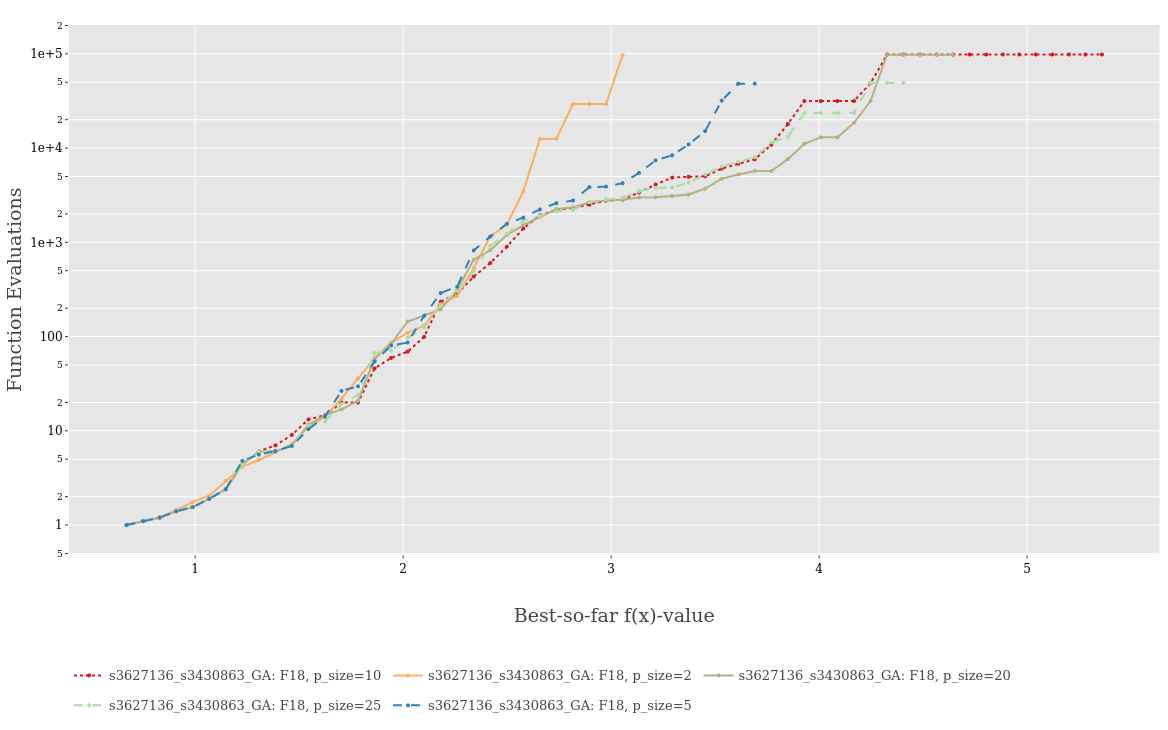
\includegraphics[width=\linewidth]{ga/f18/psize_ert.png}
        \caption{GA F18 population size fine-tuning: ERT curves. We scale y axis $\log_{10}$.}
    \end{subfigure}
    \hfill
    \begin{subfigure}[h]{0.95\linewidth}
        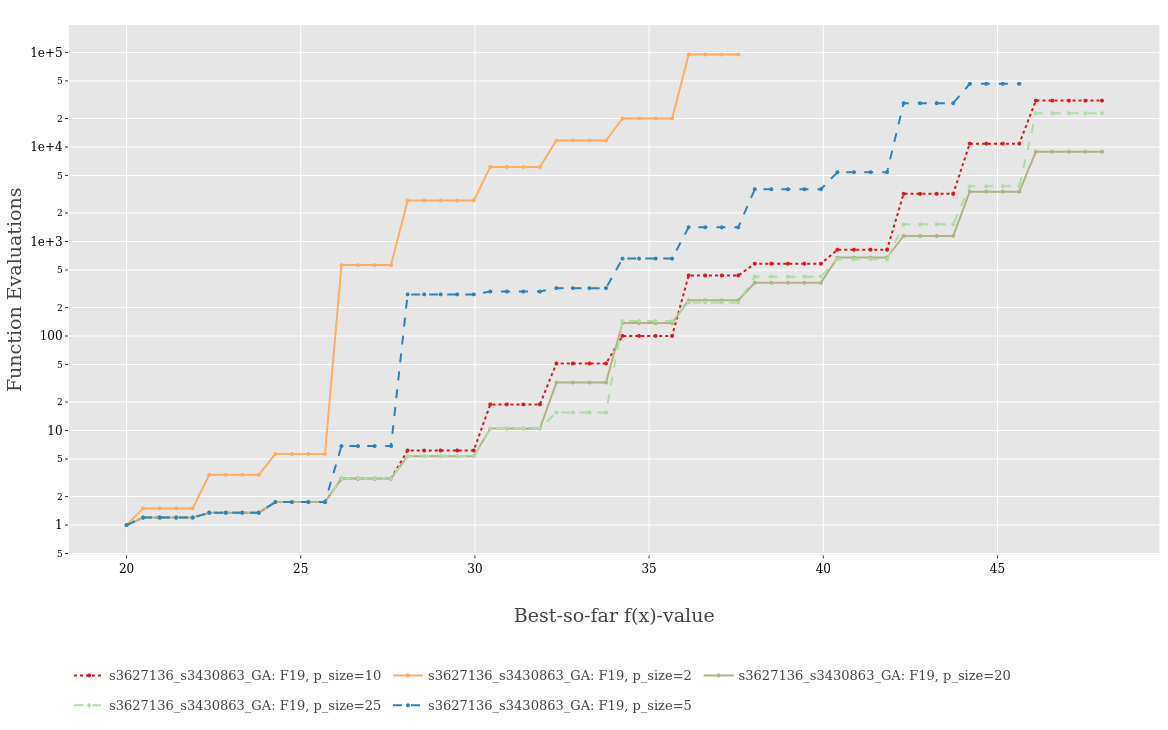
\includegraphics[width=\linewidth]{ga/f19/psize_ert.png}
        \caption{GA F19 population size fine-tuning: ERT curves. We scale y axis $\log_{10}$.}
    \end{subfigure}
    \caption{ERT curves of the genetic algorithm with various population size settings. Figures are downloaded from the IOHanalyzer.}
    \label{fig:experi-ga-psize-ert}
\end{figure}

According to Table \ref{tab:experi-ga-psize}, setting the population size to 20 achieves the best performance on the mean, median, and AUC in F18 and F19. Although it does not perform best on the max value, its overall performance exceeds other settings. ECDF curves and ERT curves support the superiority of $\mu = 20$. ECDF curves of two problems show that the small population size, like 2 or 5, prevents the algorithm from exploring a broader area in the search space. We can see that the algorithm tends to get stuck in the local optimum after the first few epochs. ERT curves also support the argument that a small population requires more budgets to reach the same level of targets. However, a larger population does not equal good performance. A population greater than 20 actually slows the convergence rate, which can be concluded from ECDF and ERT curves. Therefore, our recommendation setting of the population size is 20 for both problems.

\subsubsection{Fine-tuning: Mutation Rate}
The mutation rate controls the degree of variations the genetic algorithm introduces in each time step. According to the algorithm description in Section \ref{subsubsec:mutation}, the bit flip mutation operator accepts a constant rate at each time step. However, we think an adaptive mutation rate may be more suitable in some scenarios. Our attempts to search the appropriate mutation rate are twofold. One is trying some constant mutation rates (0.1, 0.05, $1/n=$ 0.02), and the other uses a piecewise function to adjust the mutation rate over time. Based on pilot experiments, we design a piecewise function given the budget $B = 5,000$ as follows:

\begin{align}
    p_m = 
    \begin{cases}
        0.02,\quad & B < 3000,\\
        0.1,\quad &\text{Otherwise}.
    \end{cases}
    \label{eq:ga-1}
\end{align}

The intuition behind Equation \ref{eq:ga-1} is the variation brought by the mutation should be smaller in the late stage to encourage the exploitation behavior. We refer to the usage of Equation \ref{eq:ga-1} as '\texttt{piecewise}' in tables and figures.

Table \ref{tab:experi-ga-mrate} represents the results of the mutation fine-tuning in F18 and F19. ECDF and ERT curves are shown in Figure \ref{fig:experi-ga-mrate-ecdf} and Figure \ref{fig:experi-ga-mrate-ert}.

\begin{table}[!ht]
    \centering
    \caption{Summary of statistics and AUC in mutation rate fine-tuning.}
    \label{tab:experi-ga-mrate}
    \begin{tabular}{ccccccccc}
        \toprule
        \multirow{2}[3]{*}{Mutation Rate $p_m$} &
        \multicolumn{4}{c}{\textbf{F18}} &
        \multicolumn{4}{c}{\textbf{F19}}\\
        \cmidrule(lr){2-5}
        \cmidrule(lr){6-9}
        & Mean & Max & Median & AUC & Mean & Max & Median & AUC\\
        \midrule
        0.1  & 3.01 & 3.71 & 2.94 & 0.391 & 41.9 & 44.0 & 42.0 & 0.614\\
        0.05 & 3.36 & 4.21 & 3.35 & 0.417 & 45.3 & \textbf{48.0} & \textbf{46.0} & 0.691\\
        0.02 & 3.81 & \textbf{5.36} & 3.71 & \textbf{0.496} & \textbf{46.5} & \textbf{48.0} & \textbf{46.0} & \textbf{0.763}\\
        \texttt{piecewise} & \textbf{3.90} & 4.72 & \textbf{3.89} & 0.464 & 45.0 & \textbf{48.0} & \textbf{46.0} & 0.669\\
        \bottomrule
    \end{tabular}
\end{table}

\begin{figure}[!ht]
    \centering
    \begin{subfigure}[h]{0.95\linewidth}
        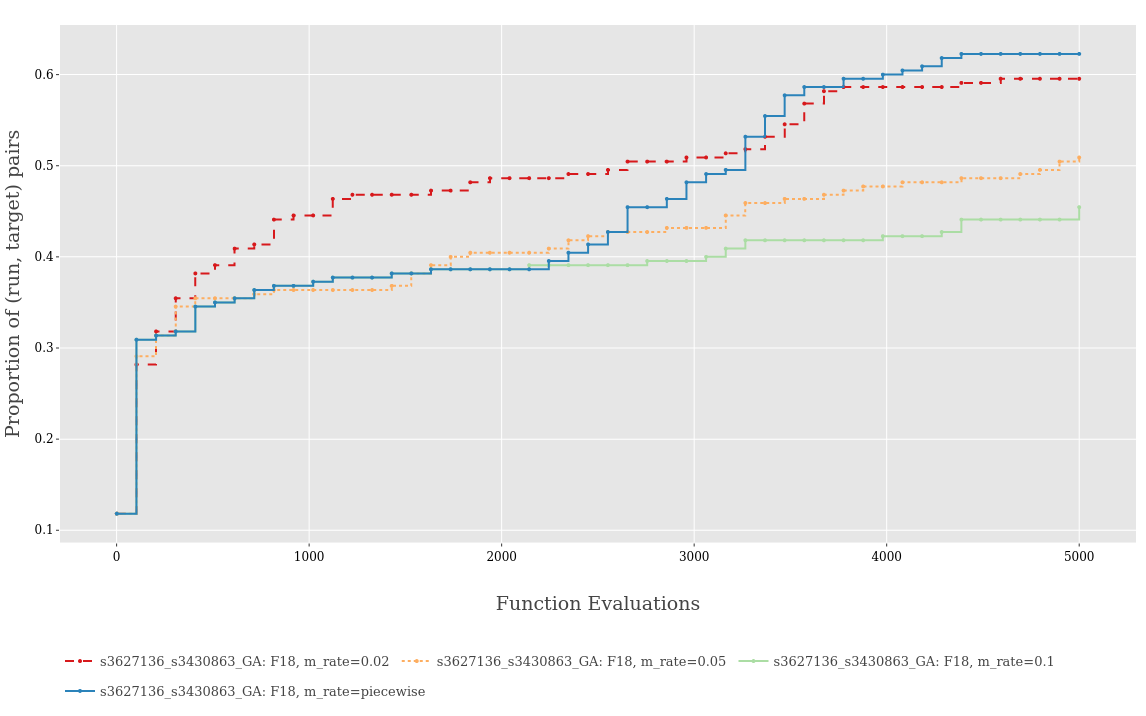
\includegraphics[width=\linewidth]{ga/f18/mrate_ecdf.png}
        \caption{GA F18 mutation rate fine-tuning: ECDF curves. $f_{\min} = 0.67, f_{\max} = 5.36, \Delta f = 0.52$.}
    \end{subfigure}
    \hfill
    \begin{subfigure}[h]{0.95\linewidth}
        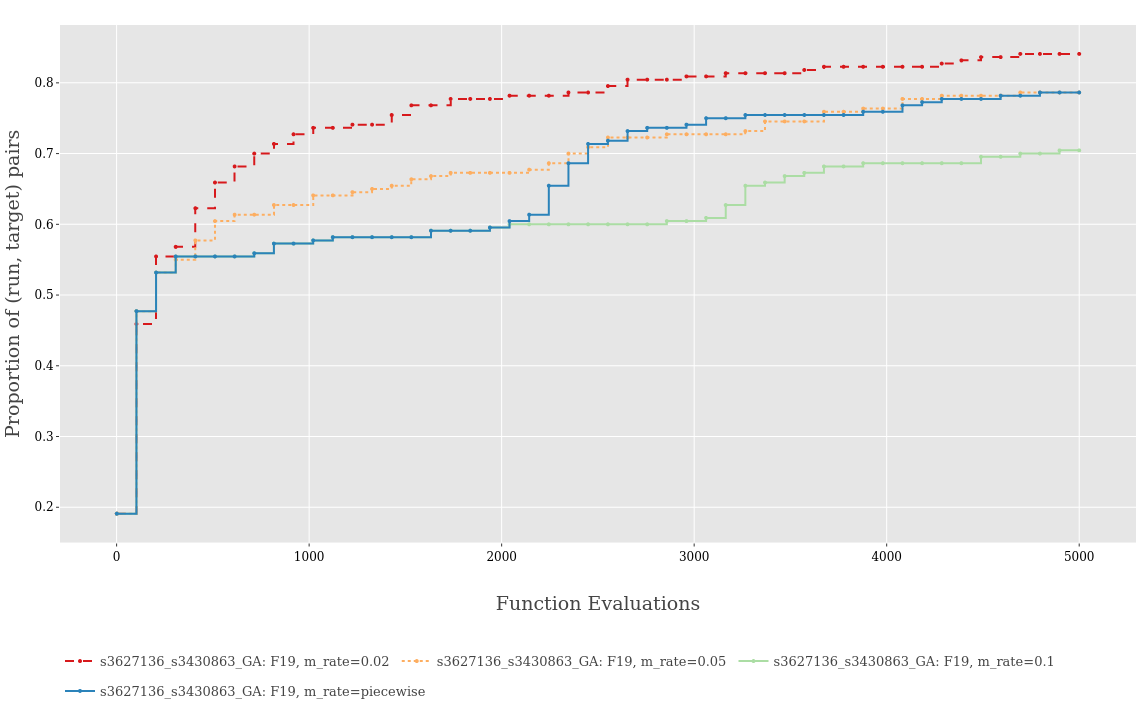
\includegraphics[width=\linewidth]{ga/f19/mrate_ecdf.png}
        \caption{GA F19 mutation rate fine-tuning: ECDF curves. $f_{\min} = 20, f_{\max} = 48, \Delta f = 3.11$.}
    \end{subfigure}
    \caption{ECDF curves of the genetic algorithm with various mutation rate settings. Figures are downloaded from the IOHanalyzer.}
    \label{fig:experi-ga-mrate-ecdf}
\end{figure}

\begin{figure}[!ht]
    \centering
    \begin{subfigure}[h]{0.95\linewidth}
        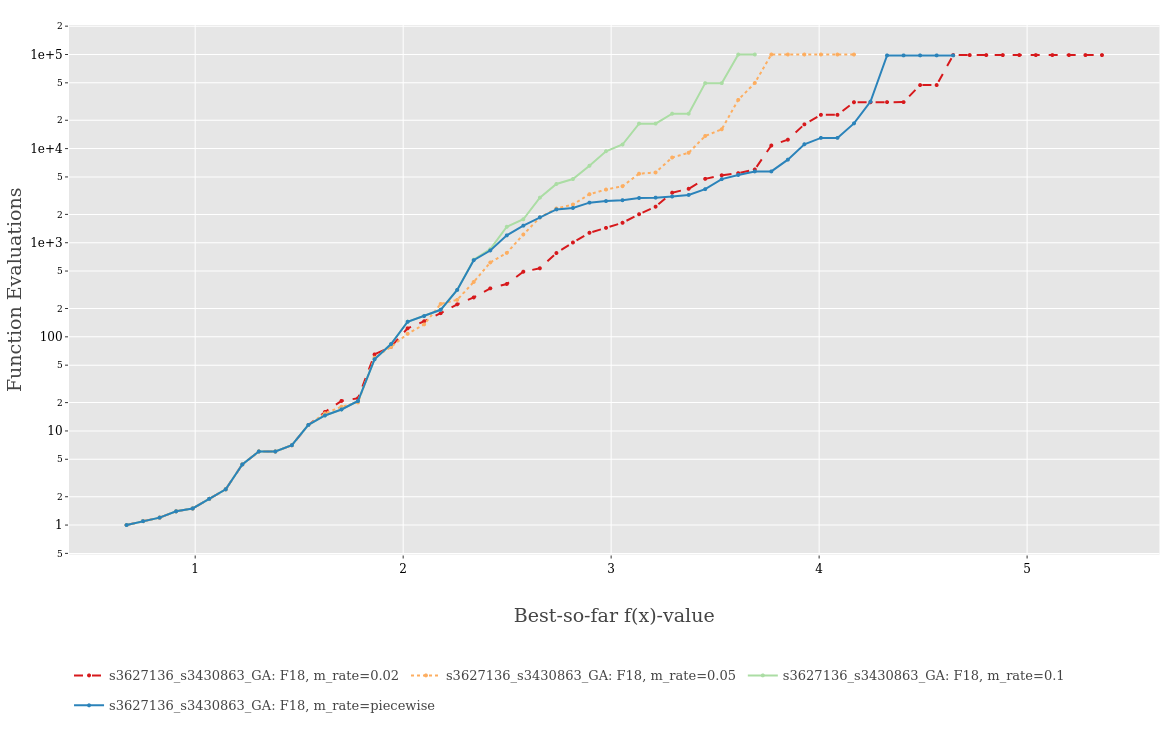
\includegraphics[width=\linewidth]{ga/f18/mrate_ert.png}
        \caption{GA F18 mutation rate fine-tuning: ERT curves. We scale y axis $\log_{10}$.}
    \end{subfigure}
    \hfill
    \begin{subfigure}[h]{0.95\linewidth}
        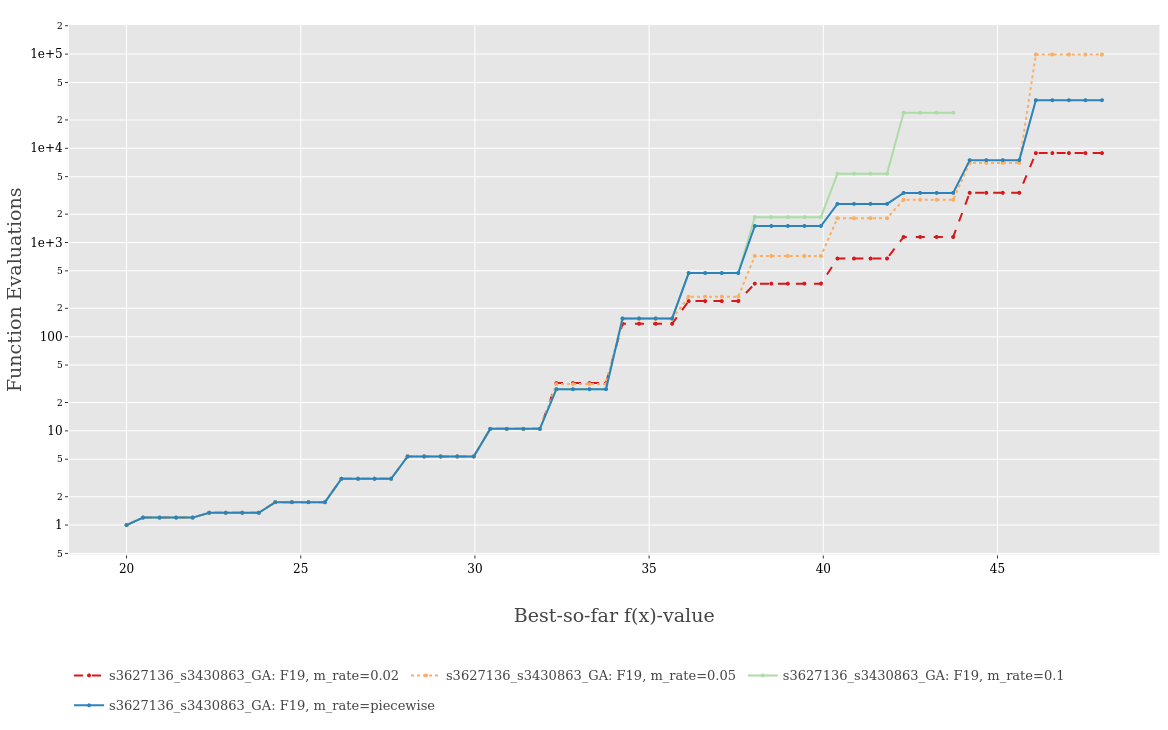
\includegraphics[width=\linewidth]{ga/f19/mrate_ert.png}
        \caption{GA F19 mutation rate fine-tuning: ERT curves. We scale y axis $\log_{10}$.}
    \end{subfigure}
    \caption{ERT curves of the genetic algorithm with various mutation rate settings. Figures are downloaded from the IOHanalyzer.}
    \label{fig:experi-ga-mrate-ert}
\end{figure}

In F18, setting $p_m = 0.02$ or using the piecewise function seems reasonable choices based on statistics and AUC values. The piecewise function performs best on the mean and median values, while $p_m = 0.02$ achieves a higher max value as well as the AUC value. However, ECDF curves suggest that the genetic algorithm is more robust with the piecewise function. Besides, ERT curves show that the piecewise function slightly accelerates the convergence rate. Hence, we conclude using the piecewise function defined by Equation \ref{eq:ga-1} is the optimal setting of the mutation rate.

Unfortunately, the same conclusion does not hold in F19. In fact, $p_m = 0.02$ outperforms all the other settings on metrics listed in Table \ref{tab:experi-ga-mrate}. ECDF and ERT curves show that $p_m = 0.02$ converges much faster than other mutation rates and achieves higher fitness values. We think the scenario defined in F19 prefers a conservative mutation rate, which means choosing $p_m = 1 / n$ can guarantee a satisfying model performance. In our case, problem dimension $n$ is 50 and $p_m$ is 0.02. 

\subsubsection{Fine-tuning: Update Ratio}
Remember that our genetic algorithm implementation only partially updates the population at each time step, as mentioned in Section \ref{subsubsec:overview}. We introduce a hyperparameter, update ratio $\theta$, to control the intensity of the update. We set the update ratio to 0.2, 0.4, 0.8, and 1.0 to find a suitable number. Notice that $\theta = 1.0$ is equivalent to the vanilla genetic algorithm. Results of the update ratio fine-tuning are summarized in Table \ref{tab:experi-ga-urate}, Figure \ref{fig:experi-ga-urate-ecdf}, and Figure \ref{fig:experi-ga-urate-ert}.

\begin{table}[!ht]
    \centering
    \caption{Summary of statistics and AUC in update ratio fine-tuning.}
    \label{tab:experi-ga-urate}
    \begin{tabular}{ccccccccc}
        \toprule
        \multirow{2}[3]{*}{Update Ratio $\theta$} &
        \multicolumn{4}{c}{\textbf{F18}} &
        \multicolumn{4}{c}{\textbf{F19}}\\
        \cmidrule(lr){2-5}
        \cmidrule(lr){6-9}
        & Mean & Max & Median & AUC & Mean & Max & Median & AUC\\
        \midrule
        0.2 & 3.53 & 4.58 & 3.43 & 0.418 & 44.9 & 48.0 & 45.0 & 0.686 \\
        0.4 & \textbf{3.90} & \textbf{4.72} & \textbf{3.89} & \textbf{0.464} & \textbf{46.5} & \textbf{48.0} & \textbf{46.0} & \textbf{0.763} \\
        0.8 & 3.35 & 4.21 & 3.28 & 0.443 & 42.6 & 46.0 & 42.0 & 0.698 \\
        1.0 & 2.99 & 3.71 & 2.94 & 0.413 & 42.3 & 46.0 & 42.0 & 0.689 \\
        \bottomrule
    \end{tabular}
\end{table}

\begin{figure}[!ht]
    \centering
    \begin{subfigure}[h]{0.95\linewidth}
        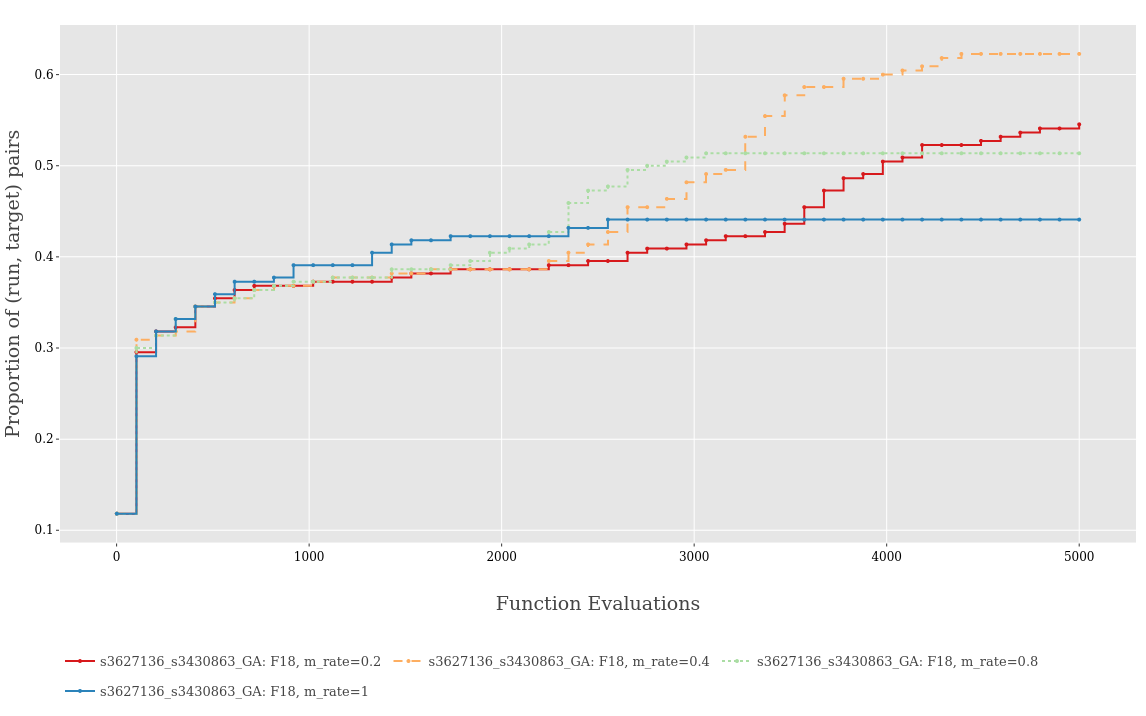
\includegraphics[width=\linewidth]{ga/f18/urate_ecdf.png}
        \caption{GA F18 update ratio fine-tuning: ECDF curves. $f_{\min} = 0.67, f_{\max} = 5.36, \Delta f = 0.52$.}
    \end{subfigure}
    \hfill
    \begin{subfigure}[h]{0.95\linewidth}
        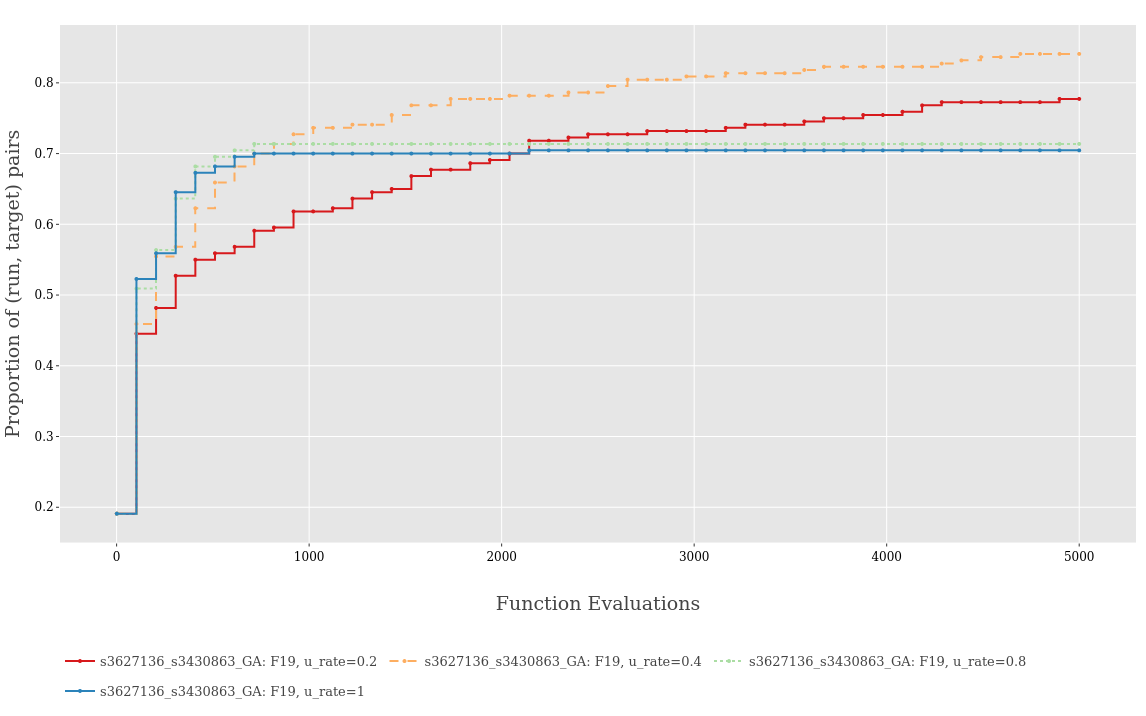
\includegraphics[width=\linewidth]{ga/f19/urate_ecdf.png}
        \caption{GA F19 update ratio fine-tuning: ECDF curves. $f_{\min} = 20, f_{\max} = 48, \Delta f = 3.11$.}
    \end{subfigure}
    \caption{ECDF curves of the genetic algorithm with various update ratio settings. Figures are downloaded from the IOHanalyzer.}
    \label{fig:experi-ga-urate-ecdf}
\end{figure}

\begin{figure}[!ht]
    \centering
    \begin{subfigure}[h]{0.95\linewidth}
        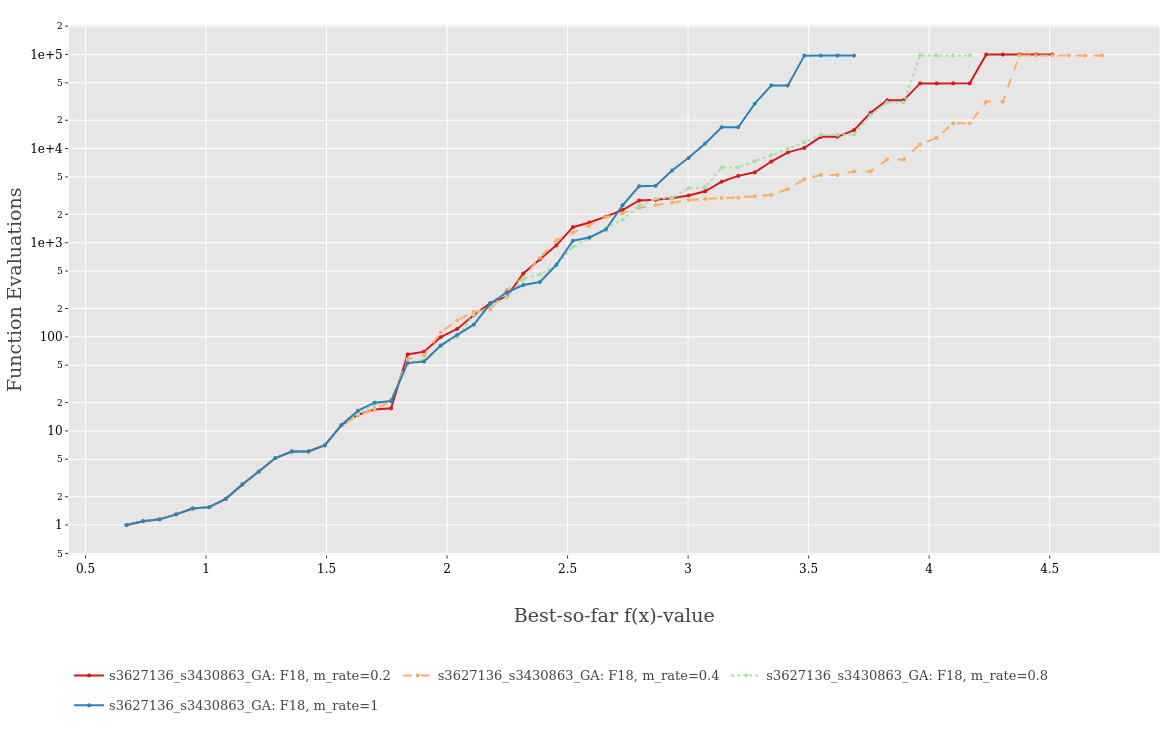
\includegraphics[width=\linewidth]{ga/f18/urate_ert.png}
        \caption{GA F18 update ratio fine-tuning: ERT curves. We scale y axis $\log_{10}$.}
    \end{subfigure}
    \hfill
    \begin{subfigure}[h]{0.95\linewidth}
        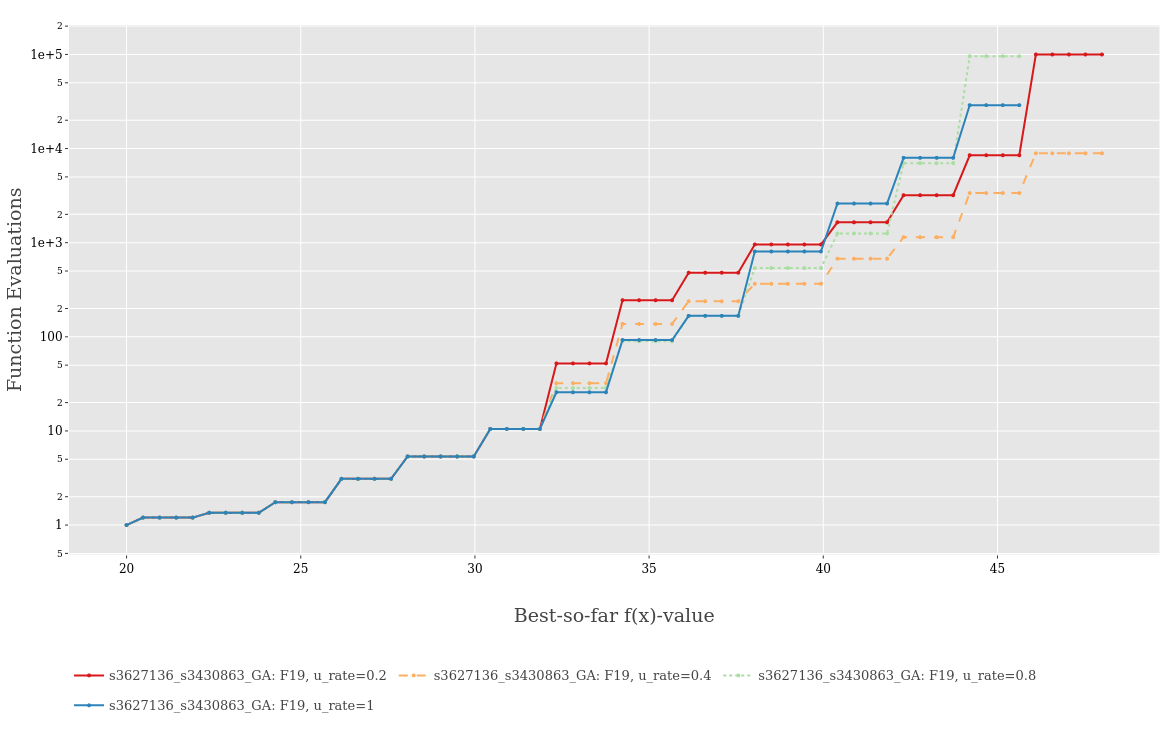
\includegraphics[width=\linewidth]{ga/f19/urate_ert.png}
        \caption{GA F19 update ratio fine-tuning: ERT curves. We scale y axis $\log_{10}$.}
    \end{subfigure}
    \caption{ERT curves of the genetic algorithm with various update ratio settings. Figures are downloaded from the IOHanalyzer.}
    \label{fig:experi-ga-urate-ert}
\end{figure}

Results validate that the update ratio is an important influencing factor of algorithm performance. Using the setting $\theta = 0.4$ obtains the best performance on all metrics in both F18 and F19. ECDF and ERT curves also support the observation that updating nearly half of the population is an effective strategy. It is worth mentioning that the vanilla genetic algorithm ($\theta = 1.0$) actually performs poorly on both problems. It is consistent with our argument in Section \ref{subsubsec:overview} that the budget $B = 5,000$ is insufficient for the vanilla genetic algorithm to converge under the problem dimension $n = 50$.

\subsubsection{Final Results}
We run the genetic algorithm 20 times on F18 and F19 with the best hyperparameter settings we have found during the fine-tuning. We summarize the final results of our implementation of the genetic algorithm as follows:

\begin{itemize}
    \item \textbf{F18}
        \begin{itemize}
            \item Hyperparameter settings: random seed $42$, budget $B = 5,000$, problem dimension $n = 50$, tournament size $t_k = 20$, tournament probability $p_k = 0.8$, population size $\mu = 20$, mutation rate using the piecewise function defined by Equation \ref{eq:ga-1} (In our code implementation, just set the mutation rate to a negative float. The program will automatically switch to the piecewise function), update ratio $\theta = 0.4$.
            \item Statistics: the averaged best-found fitness $f(x)$ = 3.90, the median of best-found fitness $f(x)$ = 3.89, the maximum of best-found fitness $f(x)$ = 4.72.
            \item AUC: 0.464.
        \end{itemize}
    \item \textbf{F19}
        \begin{itemize}
            \item Hyperparameter settings: random seed $42$, budget $B = 5,000$, problem dimension $n = 50$, tournament size $t_k = 20$, tournament probability $p_k = 0.8$, population size $\mu = 20$, mutation rate $p_m = 0.02$, update ratio $\theta = 0.4$.
            \item Statistics: the averaged best-found fitness $f(x)$ = 46.5, the median of best-found fitness $f(x)$ = 46.0, the maximum of best-found fitness $f(x)$ = 48.0.
            \item AUC: 0.763.
        \end{itemize}
\end{itemize}

ECDF and ERT curves are the same as those in Figure \ref{fig:experi-ga-urate-ecdf} and Figure \ref{fig:experi-ga-urate-ert} with the update ratio $\theta = 0.4$. We do not plot them again to conserve space. All fine-tuning experiments and the final results of the genetic algorithm can be easily reproduced by running the source code file \texttt{s3627136\_s3430863\_GA.py} in the terminal, i.e., \texttt{python s3627136\_s3430863\_GA.py}. Our final GA results of F18 and F19 are saved in \textbf{run} and \textbf{run-1} zip files respectively.

\subsection{Evolutionary Strategy}
\subsubsection{ES Fine-tuning: Population Size}

Population size denotes the number of elite individuals selected in the current generation and is also used to recombine the offspring in the next generation. We compare the algorithm performance by setting the population size to 2, 5, 10, 20, 50.  A larger population size can generate offspring diversity, increasing the probability of finding the optimal solution. In addition, the larger parent should generate more offspring to leverage its diversity advantage. Therefore, we did not use a fixed offspring number but set the $\lambda_{rate} = 2$, which means each population will generate offspring twice its size. The mutation step size $\sigma$ is set as 0.5 in this experiment. Table \ref{tab:experi-es-psize} shows the results of our experiment. Figure \ref{fig:experi-es-psize-ecdf} and Figure \ref{fig:experi-es-psize-ert} show ECDF and ERT curves, respectively.

\begin{table}[!ht]
    \centering
    \caption{Summary of statistics and AUC in ES population size fine-tuning.}
    \label{tab:experi-es-psize}
    \begin{tabular}{ccccccccc}
        \toprule
        \multirow{2}[3]{*}{Population Size $\mu$} &
        \multicolumn{4}{c}{\textbf{F18}} &
        \multicolumn{4}{c}{\textbf{F19}}\\
        \cmidrule(lr){2-5}
        \cmidrule(lr){6-9}
        & Mean & Max & Median & AUC & Mean & Max & Median & AUC\\
        \midrule
        2   & 3.35 & 4.10 & 3.31 & 0.782 & 42.3  & 46.0 & 42.0 & 0.647\\
        5   & 3.48 & 3.89 & \textbf{3.54} & \textbf{0.804} & 42.9  & 46.0 & 44.0 & 0.663\\
        10  & \textbf{3.61} & \textbf{4.86} & \textbf{3.54} & 0.759 & 43.0 & 46.0 & 43.0 & 0.659\\
        20  & 3.18 & 4.45 & 3.02 & 0.677 & 44.5  & \textbf{48.0} & 44.0 & \textbf{0.684}\\
        50  & 2.77 & 3.18 & 2.75 & 0.622 & \textbf{45.4 } & \textbf{48.0} & \textbf{46.0} & 0.648\\
        \bottomrule
    \end{tabular}
\end{table}

Table \ref{tab:experi-es-psize} demonstrates that a population size of $\mu = 10$ achieved the best statistical performance, while $\mu = 5$ resulted in the best AUC value on F18. Both ECDF and ERT curves indicate that $\mu = 10$ leads to faster and more stable convergence with better fitness. It is worth noting that a population size of $\mu = 50$ performed the worst. The reason could be this large population size leads to excessive exploration, which decreases the convergence speed in this problem. 

In contrast, for problem F19, the best statistical results are obtained with $\mu = 50$ with considerable AUC. This suggests that for problem F19, we should explore a wider search space. The ECDF and ERT also demonstrate this trend, as the population size of 50 converges smoothly towards the optimal.

In contrast, for problem F19, the best statistical results are obtained with $\mu = 50$ with considerable AUC. This suggests that for problem F19, we should explore a wider search space. The ECDF and ERT also demonstrate this trend, as the population size of 50 converges smoothly towards the optimal solution.

Therefore, we suggest use $\mu = 10$ for F18 and $\mu = 50$ for F19.

\begin{figure}[!ht]
    \centering
    \begin{subfigure}[h]{0.95\linewidth}
        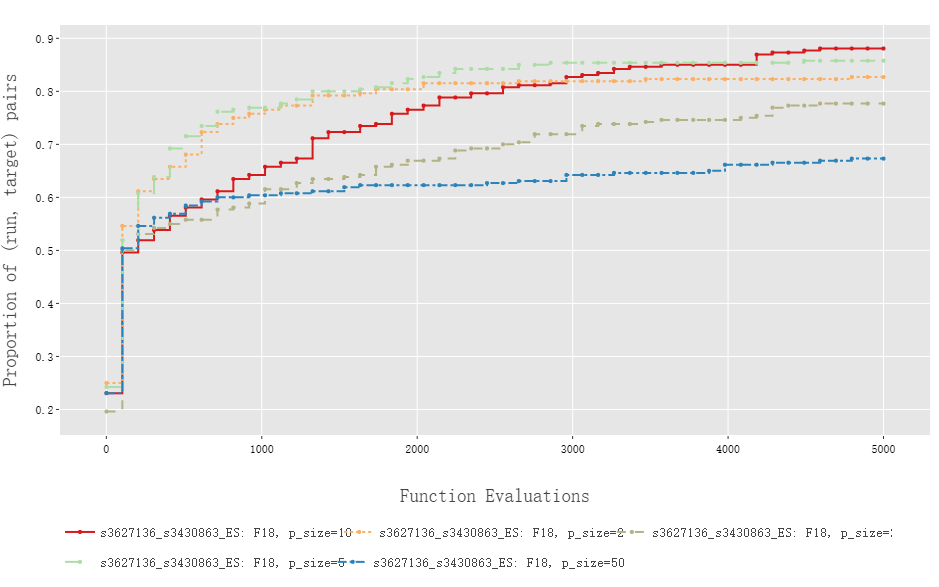
\includegraphics[width=\linewidth, height=10cm]{es/f18/ECDF18ps.png}
        \caption{ES F18 population size fine-tuning: ECDF curves. $f_{\min} = 0.4, f_{\max} = 3.83, \Delta f = 0.29$.}
    \end{subfigure}
    \hfill
    \begin{subfigure}[h]{0.95\linewidth}
        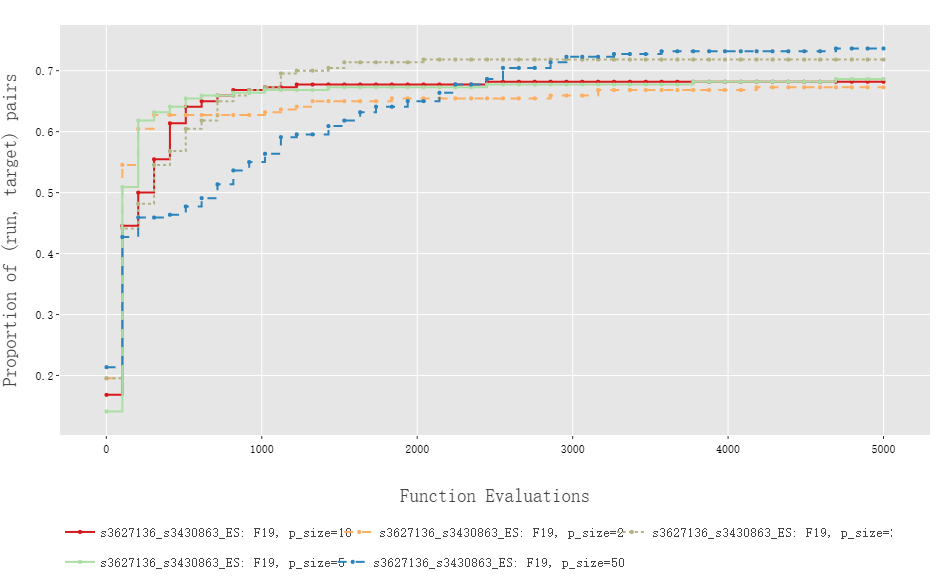
\includegraphics[width=\linewidth, height=10cm]{es/f19/ECDF19ps.png}
        \caption{ES F19 population size fine-tuning: ECDF curves. $f_{\min} = 20, f_{\max} = 50, \Delta f = 3.33$.}
    \end{subfigure}
    \caption{ECDF curves of the evolution strategies with various mutation step size settings. Figures are downloaded from the IOHanalyzer.}
    \label{fig:experi-es-psize-ecdf}
\end{figure}

\begin{figure}[!ht]
    \centering
    \begin{subfigure}[h]{0.95\linewidth}
        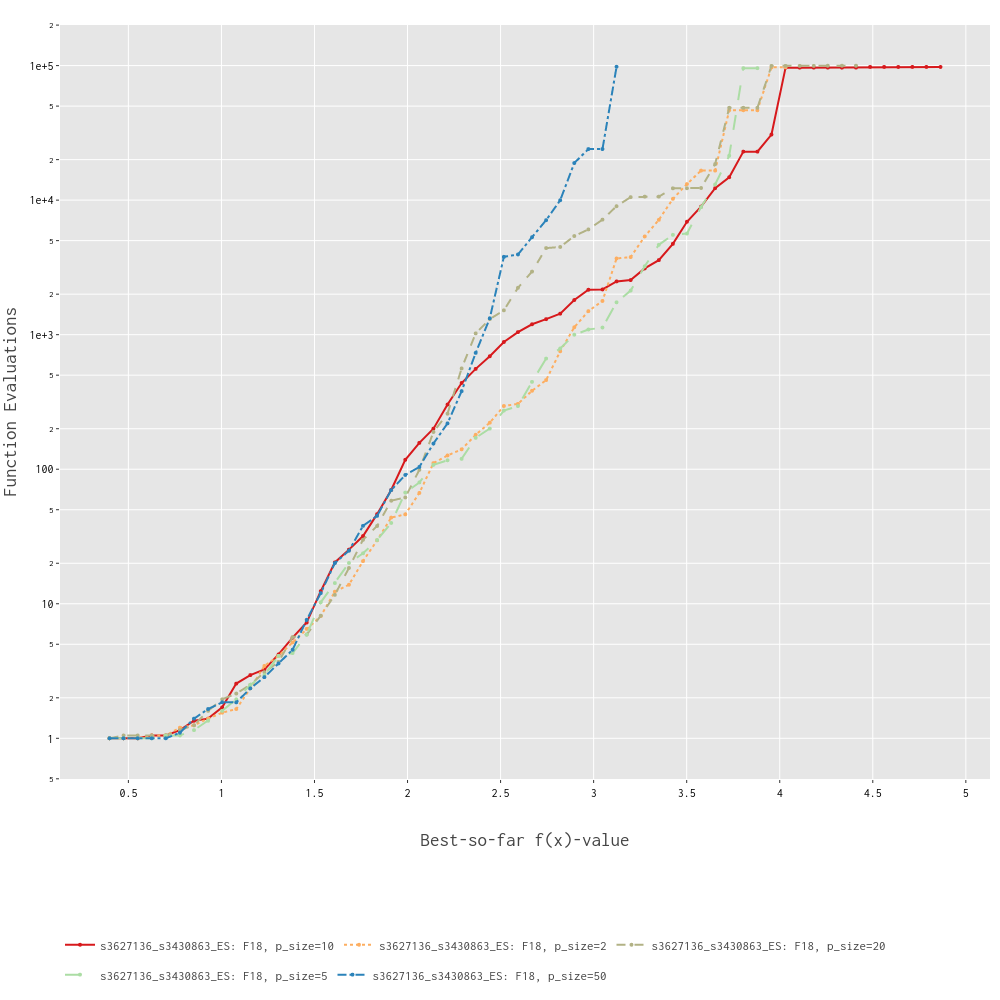
\includegraphics[width=\linewidth, height=10cm]{es/f18/ERT18ps.png}
        \caption{ES F18 population size fine-tuning: ERT curves. We scale y axis $\log_{10}$.}
    \end{subfigure}
    \hfill
    \begin{subfigure}[h]{0.95\linewidth}
        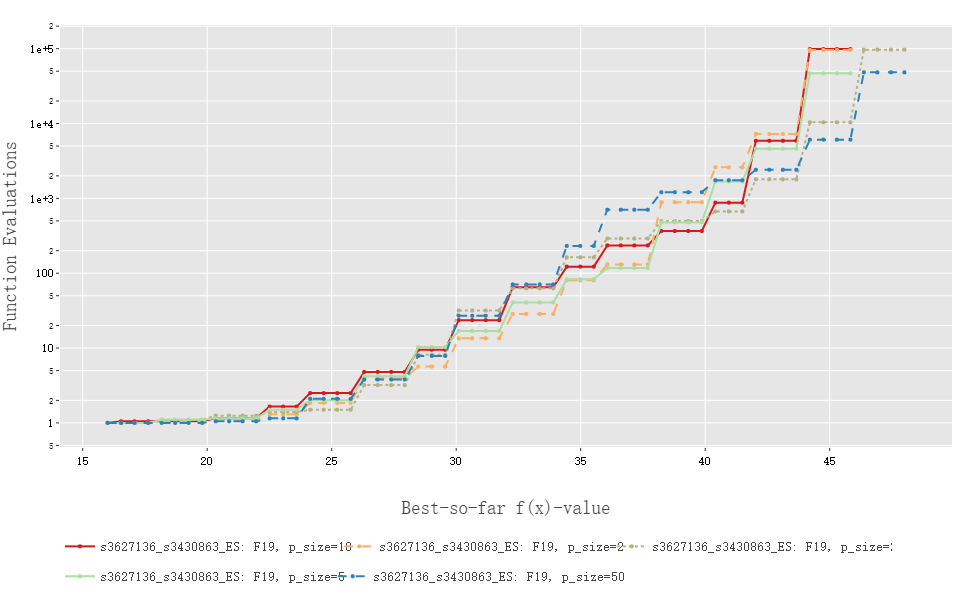
\includegraphics[width=\linewidth, height=10cm]{es/f19/ERT19ps.png}
        \caption{ES F19 population size fine-tuning: ERT curves. We scale y axis $\log_{10}$.}
    \end{subfigure}
    \caption{ERT curves of the evolution strategies with various mutation step size settings. Figures are downloaded from the IOHanalyzer.}
    \label{fig:experi-es-psize-ert}
\end{figure}

\subsubsection{ES Fine-tuning: Mutation Step Size}

The mutation step size $\sigma$ controls the perturbation extent of the individual. A larger $\sigma$ allows individuals to explore the search space faster but may cause them to skip the optimal solutions. If the mutation step size is too small, the algorithm could converge slowly and land into the local optima. In this experiment, we set the $\sigma$ to 0.1, 0.3, 0.5, 0.7, 0.9. Setting the $\mu = 20$ and $\lambda_{rate} = 2$. The statistic and AUC results shown in Table \ref{tab:experi-es-ssize}, Figure \ref{fig:experi-es-ssize-ecdf} and Figure \ref{fig:experi-es-ssize-ert} show ECDF and ERT curves, respectively.


\begin{table}[!ht]
    \centering
    \caption{Summary of statistics and AUC in ES mutation step size fine-tuning.}
    \label{tab:experi-es-ssize}
    \begin{tabular}{ccccccccc}
        \toprule
        \multirow{2}[3]{*}{Step size $\sigma$} &
        \multicolumn{4}{c}{\textbf{F18}} &
        \multicolumn{4}{c}{\textbf{F19}}\\
        \cmidrule(lr){2-5}
        \cmidrule(lr){6-9}
        & Mean & Max & Median & AUC & Mean & Max & Median & AUC\\
        \midrule
        0.1  & 3.21 & 4.10 & 3.14 & 0.736 & 41.4 & 44.0 & 42.0 & 0.615 \\
        0.3  & \textbf{3.57} & 4.33 & \textbf{3.66} & \textbf{0.738} & 43.6 & 46.0 & 44.0 & 0.667\\
        0.5  & 3.52 & 4.45 & 3.58 & 0.699 & 44.2 & \textbf{48.0} & 44.0 & 0.674\\
        0.7  & 3.05 & 4.58 & 2.83 & 0.652 & \textbf{45.1} & \textbf{48.0} & \textbf{46.0} & \textbf{0.686}\\
        0.9  & 2.89 & \textbf{5.02} & 2.64 & 0.623 & 45.0 & \textbf{48.0} & 44.0 & 0.681\\
        \bottomrule
    \end{tabular}
\end{table}

To F18, $\sigma=0.3$ produced the best results in all evaluations except for the maximum value. In the ERT experiment, the curve of $\sigma=0.5$ produced better results but converged slower than $\sigma=0.3$. When using $\sigma=0.9$ as the step size, the mean, median, and AUC values were worst, despite achieving a high maximum value of $5.02$. As we mentioned, the excessive search speed leads to the optimal solution being skipped. 

To the problem F19, The value of $\sigma=0.7$ produced impressive results in all measurements. This trend was also reflected in the ECDF and ERT curves. It's worth mentioning that $\sigma=0.9$ resulted in sub-optimal results for this problem, indicating that the algorithm needs to explore a larger search space to solve F19. This conclusion aligns with our findings in the population size fine-tuning experiment.

Therefore, we suggest to set the $\sigma=0.3$ for F18 and $\sigma=0.7$ for F19.

\begin{figure}[!ht]
    \centering
    \begin{subfigure}[h]{0.95\linewidth}
        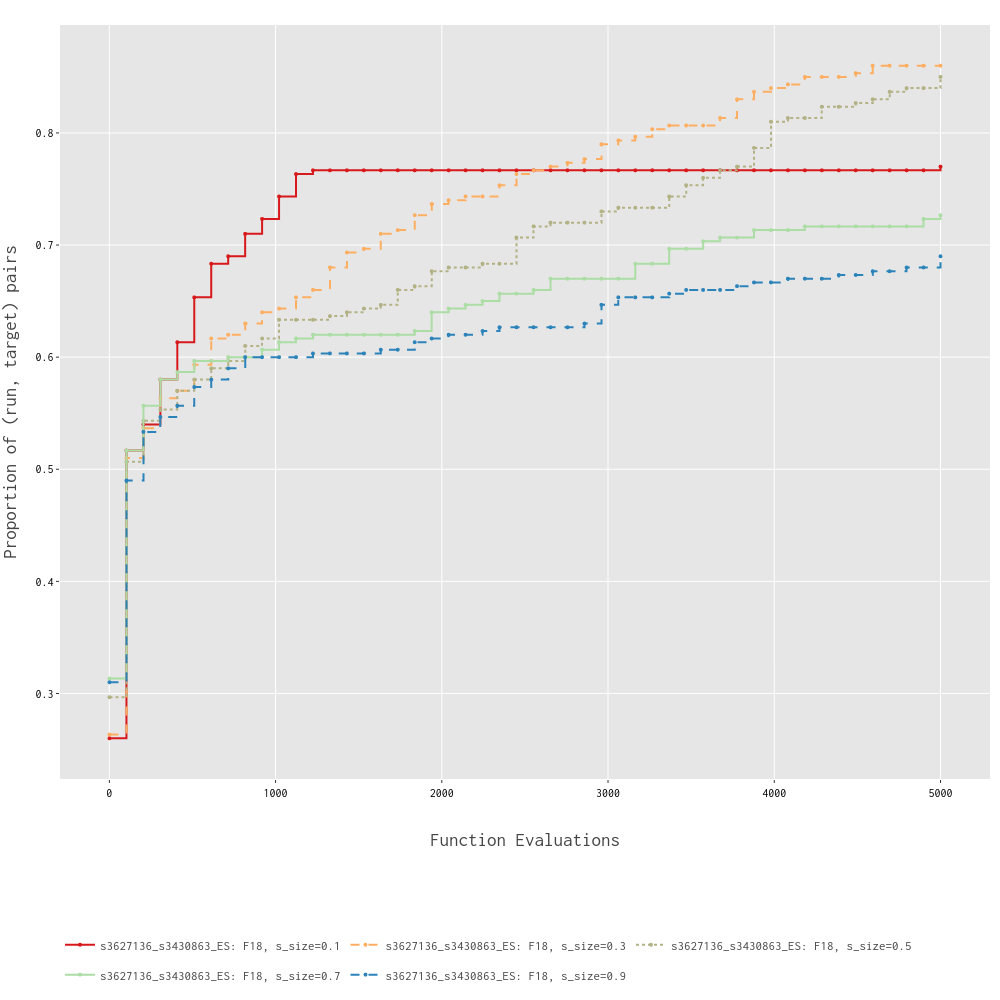
\includegraphics[width=\linewidth, height=10cm]{es/f18/ECDF18ss.png}
        \caption{ES F18 mutation step size fine-tuning: ECDF curves. $f_{\min} = 0.0, f_{\max} = 3.90, \Delta f = 0.29$.}
    \end{subfigure}
    \hfill
    \begin{subfigure}[h]{0.95\linewidth}
        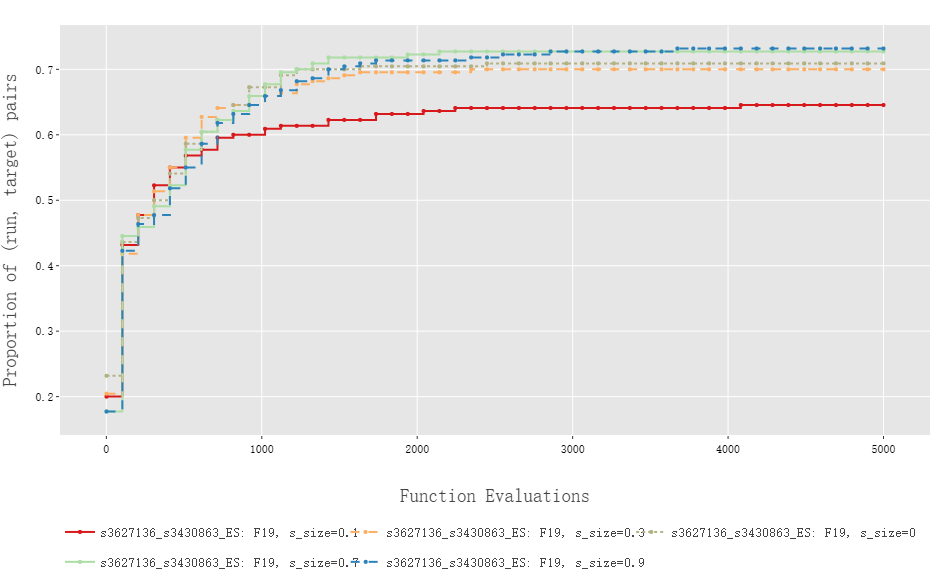
\includegraphics[width=\linewidth, height=10cm]{es/f19/ECDF19ss.png}
        \caption{ES F19 mutation step size fine-tuning: ECDF curves. $f_{\min} = 20, f_{\max} = 50, \Delta f = 3.33$.}
    \end{subfigure}
    \caption{ECDF curves of the evolution strategies with various mutation step size settings. Figures are downloaded from the IOHanalyzer.}
    \label{fig:experi-es-ssize-ecdf}
\end{figure}

\begin{figure}[!ht]
    \centering
    \begin{subfigure}[h]{0.95\linewidth}
        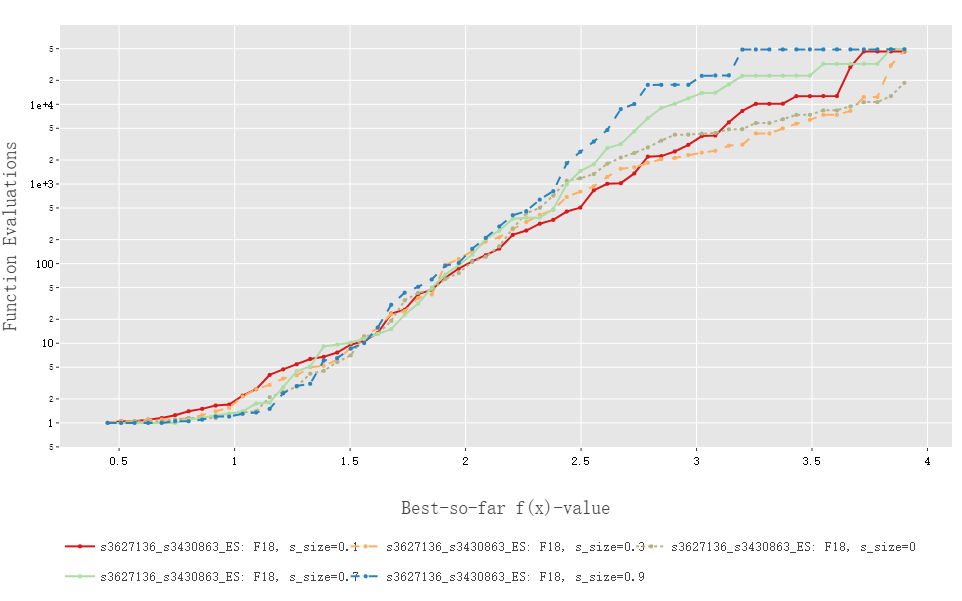
\includegraphics[width=\linewidth, height=10cm]{es/f18/ERT18ss.png}
        \caption{ES F18 mutation step size fine-tuning: ERT curves. We scale y axis $\log_{10}$.}
    \end{subfigure}
    \hfill
    \begin{subfigure}[h]{0.95\linewidth}
        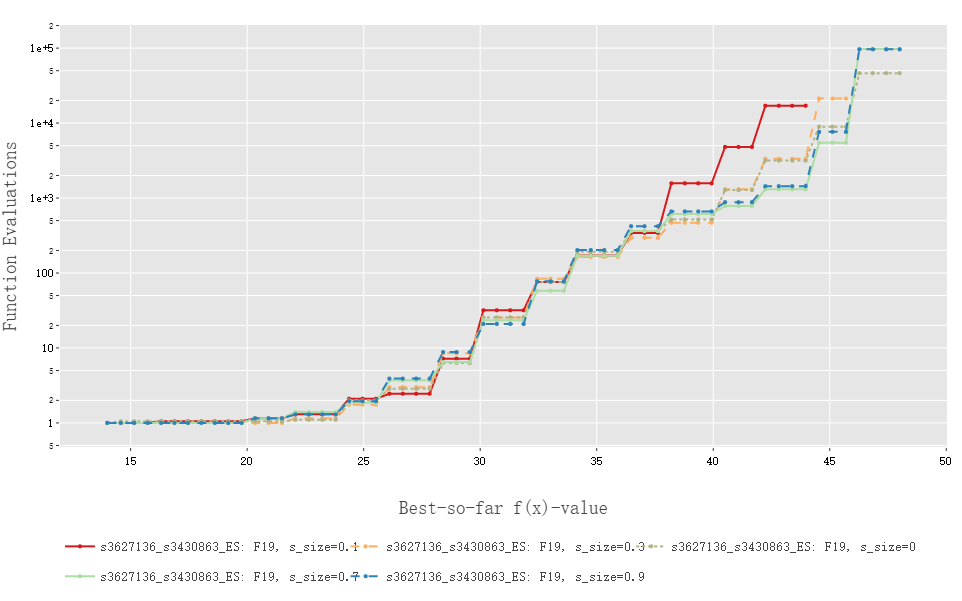
\includegraphics[width=\linewidth, height=10cm]{es/f19/ERT19ss.png}
        \caption{ES F19 mutation step size fine-tuning: ERT curves. We scale y axis $\log_{10}$.}
    \end{subfigure}
    \caption{ES ERT curves of the evolution strategies with various mutation step size settings. Figures are downloaded from the IOHanalyzer.}
    \label{fig:experi-es-ssize-ert}
\end{figure}

\subsubsection{ES Fine-tuning: Offspring size}

We explore the effects of offspring size on the algorithm's performance based on the combination of our best $\mu$ and $\sigma$. Table \ref{tab:al-es-os-hyper} shows the settings for F18 and F19. We set the $\lambda_{rate}$ to 1.5, 2, 2.5, 5, 10. Increasing the size of offspring allows the algorithm to explore the search space more extensively. However, in this assignment, due to the budget limitation, a large size of offspring leads to a significant increase in the evaluation budget per generation, causing the algorithm to fail to converge. We also compared the offspring size experiment results with the optimal results from previous experiments to determine the final parameters. The experiment ID and parameters setting are shown in Table \ref{tab:al-es-os-hyper}.


\begin{table}[!ht]
    \centering
    \caption{Hyperparameter settings of the Offspring size experiment.}
    \label{tab:al-es-os-hyper}
    \begin{tabular}{llll}
       \toprule
       \textbf{Experiment ID} & \textbf{Population size $\mu$} & \textbf{Mutation step size $\sigma$} & \textbf{Offspring size $\lambda_{rate}$}\\
       \midrule
       $F18$-$\lambda_{rate}$-experiment & 10 & 0.3 & fine-tuning\\
       $F19$-$\lambda_{rate}$-experiment & 50 & 0.7 & fine-tuning\\
       $F18$-$\mu$-optimal & 10 & 0.5 & 2.0\\
       $F18$-$\sigma$-optimal & 20 & 0.3 & 2.0\\
       $F19$-$\mu$-optimal & 50 & 0.5 & 2.0\\
       $F19$-$\sigma$-optimal & 20 & 0.7 & 2.0\\
       
       \bottomrule
    \end{tabular}
\end{table}

\begin{table}[!ht]
    \centering
    \caption{Summary of statistics and AUC in ES offspring size fine-tuning and previous optimal results.}
    \label{tab:experi-es-osize}
    \begin{tabular}{ccccccccc}
        \toprule
        \multirow{2}[3]{*}{offspring size $\lambda_{rate}$} &
        \multicolumn{4}{c}{\textbf{F18}} &
        \multicolumn{4}{c}{\textbf{F19}}\\
        \cmidrule(lr){2-5}
        \cmidrule(lr){6-9}
        & Mean & Max & Median & AUC & Mean & Max & Median & AUC\\
        \midrule
        1.5   & \underline{3.56} & \underline{4.72} & 3.42 & 0.789& 45.2& 48.0& 45.0& 0.647\\
        2.0   & 3.55 & 4.21 & \underline{3.46} &\underline{\textbf{ 0.808}}& \underline{\textbf{45.9}}& 48.0 & \underline{\textbf{46.0}} & \underline{0.652}\\
        2.5   & 3.52 & 4.21 & 3.42 & 0.776& \underline{\textbf{45.9}}& 48.0 & \underline{\textbf{46.0}} & 0.646\\
        5.0   & 3.56 & 4.33 & \underline{3.46} & 0.796& 45.8& \underline{\textbf{50.0}}& \underline{\textbf{46.0}} & 0.620\\
        10.0  & 3.47 & 4.33 & 3.42 & 0.750& 43.7& 46.0& 44.0 & 0.575\\
        \midrule
        $\mu$ optimal  & \textbf{3.61} & \textbf{4.86} & 3.54 & 0.759 & 45.4  & 48.0 & \underline{\textbf{46.0}} & 0.648\\
        $\sigma$ optimal & 3.57 & 4.33 & \textbf{3.66} & 0.738 & 45.1 & 48.0 & \textbf{46.0} & \textbf{0.686}\\
        \bottomrule
    \end{tabular}
\end{table}

In Table \ref{tab:experi-es-osize}, the first section shows the results of the $\lambda_{rate}$ experiment. The $\lambda_{rate}=2.0$ default used in previous experiments still achieves superior results for F18 and F19. The ERT Figure \ref{fig:experi-es-osize-ert} and ECDF Figure \ref{fig:experi-es-osize-ecdf} show that similar results are obtained for all parameters except the largest $\lambda_{rate}=10$.

In comparison to previous experiments, the $F18$-$\mu$-optimal continues to produce optimal statistical results for F18. While the statistical results for F19 were similar, the $F19$-$\sigma$-optimal achieved a higher AUC. Therefore, we suggest to set $\mu = 10$, $\sigma = 0.5$, $\lambda_{rate} = 2.0$ for  F18 and $\mu = 20$, $\sigma = 0.7$, $\lambda_{rate} = 2.0$ for  F19 as final results. 


\begin{figure}[!ht]
    \centering
    \begin{subfigure}[h]{0.95\linewidth}
        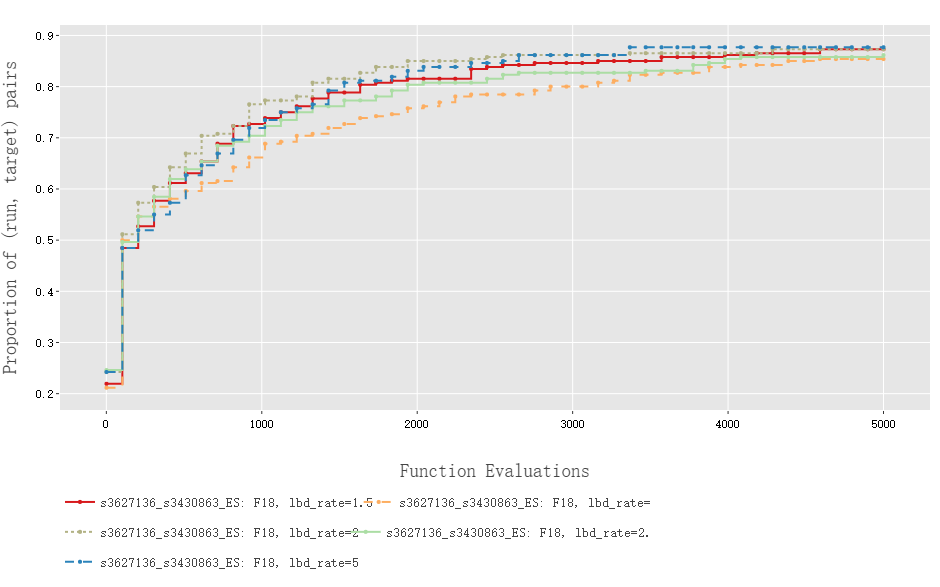
\includegraphics[width=\linewidth, height=10cm]{es/f18/ECDF18lbd.png}
        \caption{ES F18 offspring size fine-tuning: ECDF curves. $f_{\min} = 0.4, f_{\max} = 3.83, \Delta f = 0.29$.}
    \end{subfigure}
    \hfill
    \begin{subfigure}[h]{0.95\linewidth}
        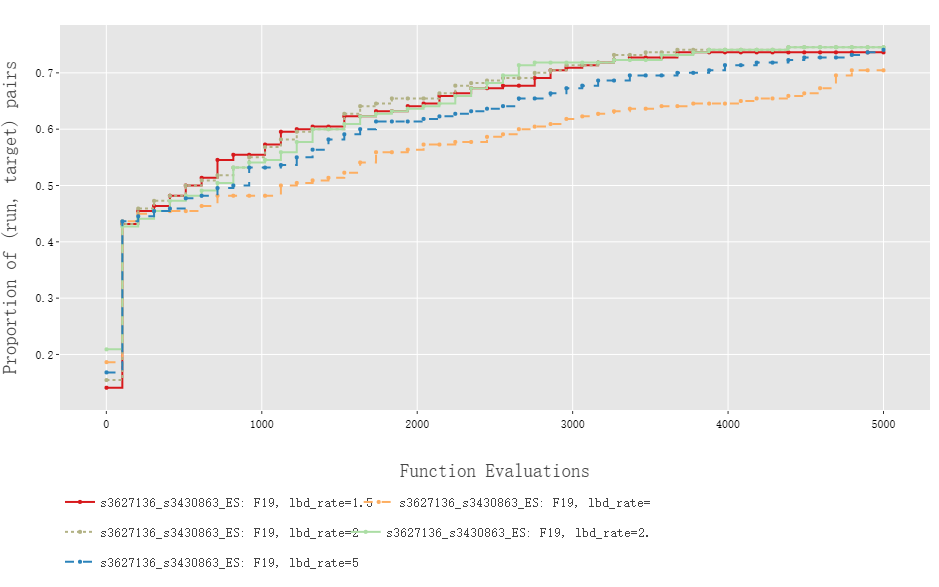
\includegraphics[width=\linewidth, height=10cm]{es/f19/ECDF19lbd.png}
        \caption{ES F19 offspring size fine-tuning: ECDF curves. $f_{\min} = 20, f_{\max} = 50, \Delta f = 3.33$.}
    \end{subfigure}
    \caption{ECDF curves of the evolution strategies with various offspring size settings. Figures are downloaded from the IOHanalyzer.}
    \label{fig:experi-es-osize-ecdf}
\end{figure}

\begin{figure}[!ht]
    \centering
    \begin{subfigure}[h]{0.95\linewidth}
        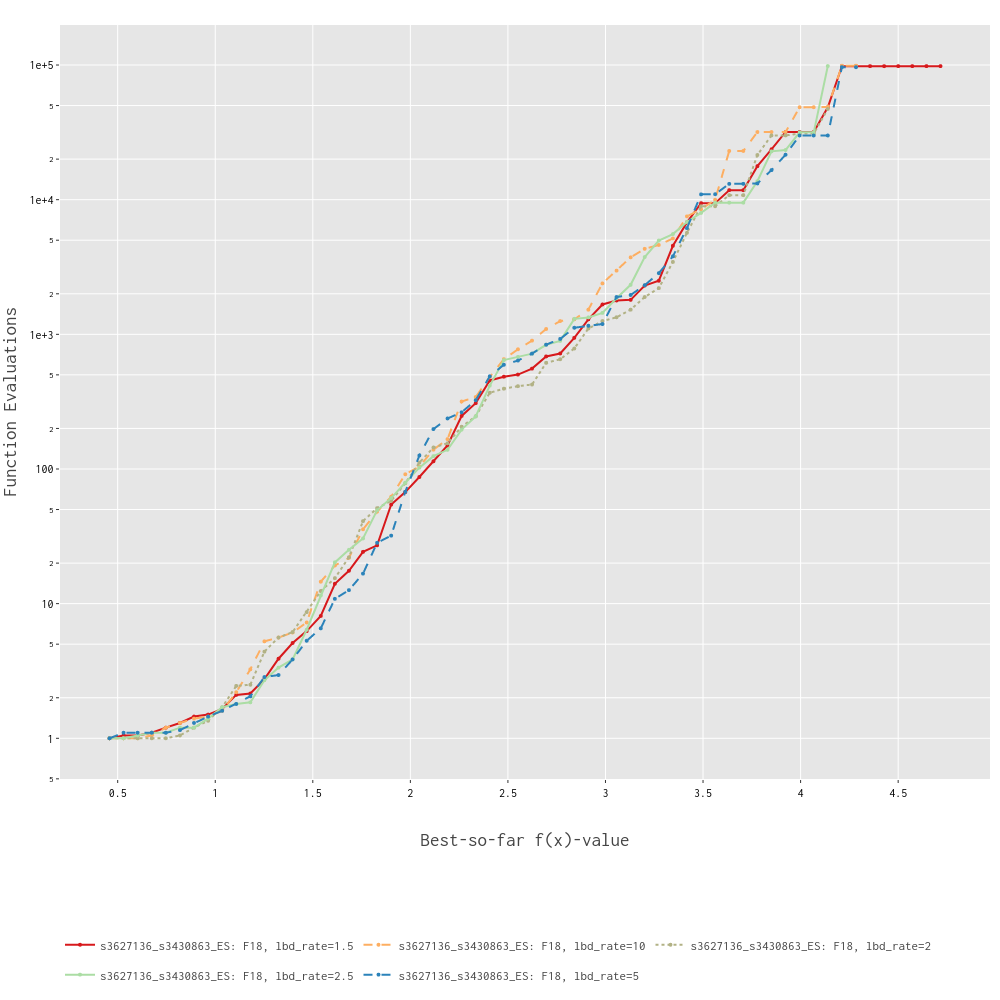
\includegraphics[width=\linewidth, height=10cm]{es/f18/ERT18lbd.png}
        \caption{ES F18 offspring size fine-tuning: ERT curves. We scale y axis $\log_{10}$.}
    \end{subfigure}
    \hfill
    \begin{subfigure}[h]{0.95\linewidth}
        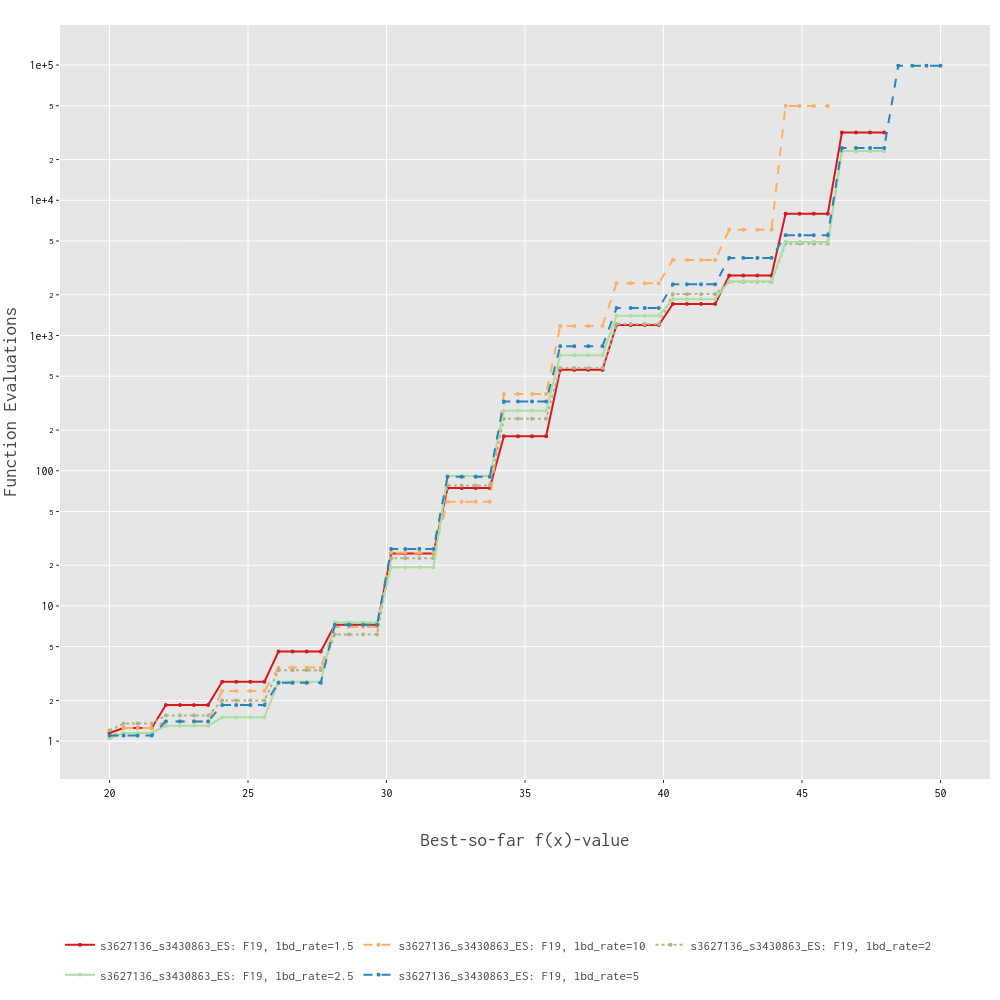
\includegraphics[width=\linewidth, height=10cm]{es/f19/ERT19lbd.png}
        \caption{ES F19 offspring size fine-tuning: ERT curves. We scale y axis $\log_{10}$.}
    \end{subfigure}
    \caption{ES ERT curves of the evolution strategies with various offspring size settings. Figures are downloaded from the IOHanalyzer.}
    \label{fig:experi-es-osize-ert}
\end{figure}

\subsubsection{ES Final Results}
We summarize the final results of our implementation of the evolution strategies as follows:

\begin{itemize}
    \item \textbf{F18}
        \begin{itemize}
            \item Hyperparameter settings: random seed $42$, budget $B = 5,000$, problem dimension $n = 50$, population size $\mu = 10$, mutation step size $\sigma = 0.5$ and offspring size $\lambda_{rate} = 2.0$.
            \item Statistics: the averaged best-found fitness $f(x)$ = 3.61, the median of best-found fitness $f(x)$ = 3.54, the maximum of best-found fitness $f(x)$ = 4.86.
            \item AUC: 0.759.
        \end{itemize}
    \item \textbf{F19}
        \begin{itemize}
            \item Hyperparameter settings: random seed $42$, budget $B = 5,000$, problem dimension $n = 50$, population size $\mu = 20$, mutation step size $\sigma = 0.7$ and offspring size $\lambda_{rate} = 2.0$.
            \item Statistics: the averaged best-found fitness $f(x)$ = 45.1, the median of best-found fitness $f(x)$ = 46.0, the maximum of best-found fitness $f(x)$ = 48.0.
            \item AUC: 0.686.
        \end{itemize}
\end{itemize}

 All fine-tuning experiments results can be reproduced by running the source code file \texttt{s3627136\_s3430863\_ES.py} in the terminal, i.e., \texttt{python s3627136\_s3430863\_ES.py}. After the script is executed, the best results of F18 correspond to the folder \textbf{data/population size p\_size=10 run}, and best results of F19 correspond to the folder \textbf{data/Step size s\_size=0.7 run-1}. All experimental results and the final results have been archived as zip files in the \textbf{data-file} folder. 


\section{Discussion and Conclusion}
\label{sec:dis&res}
In this assignment, we implement genetic algorithms and evolutionary strategies to solve the F18 and F19 problems from the IOHprofiler. We explore various search strategies and fine-tuning parameters to improve algorithm performance. In the evolutionary algorithm, we combine three classical selection algorithms in the selection phase, according to each algorithm's advantages, to balance exploitation and exploration. In addition, we fine-tune the key parameters such as population size, mutation rate and update ratio. Then, we determine the optimal parameter settings by evaluating the averaged best-found fitness, the median of best-found fitness, the maximum of best-found fitness, AUC, ECDF, and ERT. Within the evolution strategies, we initialize the population through Gaussian distribution in the real value space, then map the solutions into the binary distribution via cdf to interact with the problem. Moreover, we conduct experiments with population size, mutation step size, and offspring size to fine-tune the algorithm parameters.
 
Overall, the genetic algorithm achieves a better performance. The evolution strategies may suffer the loss from the value domain transformation. Neither algorithm is able to find the optimal solution due to budget constraints. In future research, we plan to explore more strategies and fine-tune the algorithm parameters to converge to the optimal solution with as few budgets as possible.


\bibliographystyle{unsrt}  
\bibliography{references}  

\end{document}
